\chapter{Background}

% Introduce what is planning under uncertainty
Acting under uncertainty is central to AI and robotics and has been an active area of research for decades. It
is an umbrella term which encompasses a wide spectrum of fields:  \textit{economics}, \textit{psychology}, 
\textit{cognitive science}, \textit{neuroscience}, \textit{robotics} and \textit{artificial intelligence}.
The work in this thesis relies on results from all of the aforementioned fields with varying degree.
Cognitive and neuroscience bring justification into the way we represent our beliefs and how we act accordingly. 
AI and robotics provide computational models and optimisation methods some of which are biologically inspired.
Because of the vast spectrum of topics we cannot do justice to all them and we will focus on works which are directly 
relevant to the problems we are addressing in this thesis.
In this chapter we cover the following topics in the presented order: Decision Theory (DT), Markov Decision Process (MDP), 
Partially Observable Markov Decision Process (POMDP), a literature review and the approach taken 
in this thesis.\\[0.05cm]

\begin{figure}[h]
 \centering
 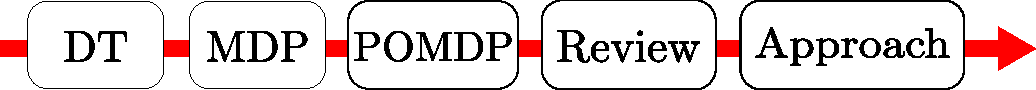
\includegraphics[width=0.9\textwidth]{./ch2-Background/Figures/chap_overview.pdf}
  \caption{Chapter outline.}
  \label{fig:ch2_outline}
\end{figure}

\begin{itemize}
 \item \textbf{Section} \ref{sec:deci_un}, introduces what is meant by taking decisions under uncertainty and what are the different 
 sources of uncertainty. We take a historical look at Decision Theory since it is the root node of all subsequent research in reasoning 
 and acting under uncertainty and provides for a good introduction to the topics which will follow.  
 \item \textbf{Section} \ref{sec:sqp},  mathematically formalises the sequential decision problem under uncertainty and is linked with Decision Theory. We derive from first principal 
 the Bellman optimal equation which is one of the most important result to date in sequential decision processes.
 \item \textbf{Section} \ref{sec:lit_rev}, provides an in depth literature review with the latest results in AI \& robotics in the subject 
of planning and acting under uncertainty. We draw attention to the different approaches to solving this problem whilst pointing out
their advantages and weaknesses.
 \item \textbf{Section} \ref{sec:approach}, summaries what has been achieved so fare, what are the open problems and how this 
 thesis contributes and complements the field. 
\end{itemize}



\section{Decisions under uncertainty}\label{sec:deci_un}
% What is the the reasoning under uncertainty planning problem
% What are all the assumptions which can be made regading the belief

%In this section we introduce and frame the problem we seek to solve in generic 
%terms. 
The main objective of reasoning under uncertainty is to find an action or sequence of
actions which will result in the most preferable outcome. There are two key attributes which can render this 
problem difficult: \textbf{stochastic actions} and \textbf{latent states}. 

Stochastic actions when applied in the same state will not always result in the same outcome. This type of uncertainty 
can arise from many sources. For instance, the outcome of chaotic systems will always lead to different results when the same action is applied
to the same initial conditions, such as the throwing of a dice or the flipping of a coin. In outdoor robotics the terrain might lead to slippage, causing 
the robot to skid, or in an underwater environment currents might drastically offset the position of an UAV. In articulated robots, the friction in the joints 
can result in an error in the end-effector position (especially true for cable driven robots).

The second source of uncertainty is when the state space cannot be determined. This arises when the sensors are not able to 
provide sufficient information to reliably estimate the state. In robotics this uncertainty can arise from inadequate or noisy sensors. 
In poor environmental conditions such as humidity, lack of light or smoke the robot can experience difficulties in 
ascertaining its position and thus in planning how to achieve a given objective.

Given these two types of uncertainty, the question is how to represent these uncertainties. The predominant approach 
is to quantify the uncertainty in terms of probabilities. For instance the application of a forward action to a wheeled robot 
will result in some probability in a new position further ahead and with a remaining probability distributed to adjacent 
regions which might have occurred due to slippage.

An observation made through the robot's sensors will result in a probability distribution over the robot's probable location.
This quantification of the action and observation uncertainty, in terms of a probability distribution over the state, must
be utilised by the agent to plan actions towards accomplishing its goal. In order to take a decision, the agent must assign a utility 
to each state weighted by the probability of its outcome and act so as to get the highest utility. The utility indicates a 
preference over the outcomes and when combined with probabilities leads to Decision Theory, which is the topic of the next section. 

\subsection{Decision theory}

The central question that Decision Theory asks is: \textit{how do we take decisions when faced with uncertain outcomes ?} To answer
such a question we need to identify the attributes which are involved when we take a decision, namely our \textbf{beliefs} and 
\textbf{desires}. Beliefs reflect a degree of knowledge we have about the world. This degree is ascertained by 
the amount of evidence we have in support of our beliefs. Epistemology studies in great detail the relationship between 
truth, beliefs and knowledge. We will not go into a philosophical discussion of their interplay, but make use of the following: 
if we have sufficient evidence in support of our beliefs and they represent the truth then we consider them to 
be \textbf{rational beliefs}. As for desires, they are linked to our disposition to take upon them. For 
example if I want to switch off my alarm clock I have to look for it in the last area I believed it to be in. 
These two attributes, beliefs and desires, are used to frame a decision problem. Early work in decision theory assumed 
that the problem was well grounded and focused on finding what \textbf{rational actions} need to be taken given our beliefs 
in order to achieve our desires. 

\begin{figure}
 \centering
 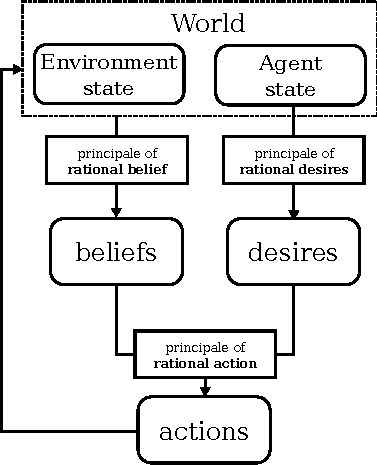
\includegraphics[width=0.5\textwidth]{/home/guillaume/Documents/Thesis/ch2-Background/Figures/cognitive_loop.pdf}
  \caption{Relation between beliefs, desires and actions and are all considered to be rational.}
\end{figure}

Early interest in such questions were typically centred around economics which included deciding an appropriate 
investment or wager for a particular gamble. It was noted that the expected monetary outcome of a gamble as a means of basing a 
decision, would often lead to a course of action which contradicts common sense. A famous example of this contradiction
is demonstrated in the St. Petersburg paradox. In this paradox a bookmaker proposes the following gamble. 
An initial pot starts with a content of \pounds2. The bookmaker proceeds to flip a fair coin until the first appearance of a 
tails which ends the game. Until the occurrence of the first tails the money in the pot doubles after every toss. Once the 
game ends the player leaves with the contents of the pot. As an avid gambler and \textbf{expected value} maximiser how much 
would one be willing to pay to enter this game ? To access, one would need to know the average payout. The amount 
of money increases by \pounds$2^{n}$, where $n$ is the number of non-final tosses and the probability of 
reaching $n$ is $1/2^{n}$. In this case the expected monetary outcome is infinite:

\begin{equation*}
\displaystyle \mathop{\mathbb{E}}_{p(\pounds)}\{\pounds\} = \underbrace{\frac{1}{2} \pounds2}_{\textrm{first toss}} + \frac{1}{4} \pounds4 + \dots = \sum\limits_{n=1}^{\infty} 
\pounds\frac{2^{n}}{2^{n}} = \pounds\infty 
\end{equation*}

So the expected gain or return for paying to enter such game is an infinite amount of money. Thus in principal if a player was
seeking to maximise his expected return value he would be willing to pay an amount close to infinity to enter the game. 
This does not seem a good decision rule; no person in the world would be willing to pay such high amounts to enter this game.

Nicolas Bernoulli proposed a solution to the problem which was later published by his brother Daniel (republished \cite{Bernoulli1954}). 
He introduced the notion of a \textbf{utility function}, and he claimed that people should base their decision on 
the expected utility instead of solely on the monetary outcome.

\begin{quote}
  \onehalfspacing% <--- Local line spacing
  ``...the value of an item must not be based on its price, but rather on the utility it yields."\par\raggedleft--- \textup{Daniel Bernoulli}
\end{quote}

The introduction of a utility function takes into account that the net worth of a person will influence their decision since 
different people (in terms of their monetary worth) will weigh the gain differently. The utility function introduced by Bernoulli 
was the logarithm of the monetary outcome $x \in X$ weighted by its probability $p(x)$ which results in an expected utility: 

\begin{equation*}\label{eq:exp_utility}
  U(x) = \displaystyle \mathop{\mathbb{E}} \{ u(x) \} = \sum_{x\in X} p(x) \underbrace{\log(x)}_{u(x)}
\end{equation*}

%Different utility functions characterise different levels of risk. When the it is concave as it for Bernoulli's utility function
%the person will be \textbf{risk-averse}, when linear \textbf{risk-neural} and convex \textbf{risk-seeking}. 
%This was the first introduction of a utility function. 

It is later in 1944 that von Neumann and Morgenstern (\cite{VonNeumann1944}) axiomised Bernoulli's utility function 
and proved that if a decision maker has a preference over a set of lotteries\footnote{the term lottery refers 
to a probability distribution in the original text.} which satisfy four axioms
(completeness, transitivity, continuity, independence) then there exists a utility function whose expectation 
preserves this preference. An agent whose decisions can be shown to maximise the vNM expected utility are said 
to be \textbf{rational} otherwise they are \textbf{irrational}.

%\begin{equation*}
% a^* = \max_a U(x|a)
%\end{equation*}


This is the theoretical basis of most economic theory. It is a \textbf{normative} model of how people should behave given uncertainty. It is also the basis of most 
if not all decision making, cogitative architectures and control policies in AI and robotics (to the best of the author's knowledge).

An aspect to keep in mind regarding the vNM model is that it is normative; it states what should be a rational decision. 
As a result it is not always consistent with human behaviour. There is great debate regarding 
the predictions made by vNM models with respect to our behaviour. There have been many studies both demonstrating divergence 
between the model's predictions and our observed behaviour but also supporting evidence that it does reflect 
the output of our decision making process. Reasons for divergence have been attributed to how people
weigh probabilities and how the decision problem is framed. But probably the most important aspect is that 
in most decisions we are faced with, the quantification and rationality of our beliefs might not be adequate
and limitations of our working memory will come into play in the final decision.

Nevertheless vNM agents are predominantly used in AI and robotics as a means of implementing 
decision making processes or in control policies. In psychology and cogitative science vNM agents
are a used for comparing human behaviour against an optimal strategy (by optimal we mean it is rational in 
the vNM sense). It is important to remember the origins and assumptions underlying the models that 
are used to represent control policies or cognitive architectures implemented into robotic systems or 
software agents.

% (see prescriptive models(\cite{Kahneman79prospecttheory}). 
% vNM is concerned with a one shot only decision, but what if we have to take a sequence of decisions ? What 
% happens then ?
% How is the uncertainty quantified ? Answer: probability theory
% How does the agent make a decision ? He must assigned a preference to the outcome of various actions
% Utility theory and combined with probability lead to decision theory.
% Speak about the historical context of plannig un
% Uncertainty and rational actions
% vNM theorem is limited to evaluation options that come with an 
% objective probability distribution over outcomes.
% a situation decision theoriests and economists often describe 
% as ''choice under risk``
% The utility function represents the agents desires.
% so the probability function represents her beliefs.
% The theories are referred to collectively as subjective expected utility (SEU).
% How is decision theory used in robotics ?
% POMDPs provide a rich framework for sequential decision-making under uncertainty in stochastic domains.
% Solving a POMDP is often intractable.

\begin{table}
\begin{center}
\renewcommand{\arraystretch}{1.5}
\begin{tabular}{|l|p{9cm}|} 
\hline
    \textbf{Notation} 			 	& \textbf{Definitions} \\ \hline\hline
    $x_t \in \mathbb{R}^3$ 		 	& Cartesian state space position of the agent.\\
    $y_t \in \mathbb{R}^{M}$		 	& Observation/measurement from the agents sensors.\\
    $a_t \in \mathbb{R}^3$		 	& Action, usually the Cartesian velocity of the end-effector of the agent.\\
    $X,Y,A$				 	& State, observation and action random variables where $x$, $y$ and $a$ are realisation.\\
    $p(x_t)$ 					& Short hand notation for a probability density function, $p_{X}(x_t)$.\\
    $x_{0:t}$					& $\{x_0,x_1,\cdots,x_{t-1},x_t\}$, history up to time $t$.\\
    $p(x_t|y_{0:t},a_{0:t})$	 		& Filtered probability distribution over the state space given the action and observation history.\\
    $b_t \in \mathbb{R}^{L}$			& Belief state, a function of the filtered distribution 
						 $b(p(x_t|y_{0:t},a_{0:t}))$ which will be written as $b_t$ for simplicity.\\
    $\policy(a_t|\cdot)$ 			& Probabilistic policy, $a_t \sim \pi_{\boldsymbol{\theta}}(a_t|\cdot)$ \\
    $u(x) \in \mathbb{R}$			& Utility function, returns the utility of being in state $x$. It can also be dependent on the action, $r(x,a)$.\\
    $\gamma \in [0,1)$				& Discount factor, the closer to one the more the later utilities are considered. When set to zero, only immediate rewards are 
						  considered which would result in a myopic greedy agent.\\
    $p(x_{t+1}|x_t,a_t)$			& State transition function, returns the likelihood/probability of reaching state $x_{t+1}$ given that action $a_t$ is applied in state $x_t$.\\	
    $p(y_t|x_t)$				& Observation/measurement model, returns the likelihood/probability of observing $y_t$ given that the agent is in state $x_t$.\\
    $\tau(b_{t-1}(x),u_{t-1},y_t)$		& Updates a belief given a motion and observation. It makes use of both the motion and observation functions. The state space estimation function, $\tau$, can be any kind of state space filter such as an Extended Kalman Filter (EKF) or a Particle Filter (PF).
    \\ \hline
\end{tabular}
\end{center}
\caption{Definition of common variables used.}
\label{tab:notation}
\end{table}


\section{Sequential decision making}\label{sec:sqp}

When Decision Theory is brought up, we are usually referring to a one shot non-temporal decision. 
However many interesting decision problems are sequential. In such situations, we must consider 
the effect current decisions will have on future decisions. Expected utility theory (part of Decision Theory) is 
extendable to a temporal decision problem. There are however two subtle but important 
differences between the temporal and non-temporal decision problems. The first difference is the utility. In the one 
time step problem an outcome has one utility assigned to it, $u(x)$. In the temporal decision problem a utility has to 
be assigned to a sequence of outcomes, $u(x_{0:T})$, where $T$ is the number of sequential decisions taken. The utility 
of a sequence is the sum of the individual utilities. However if the decision problem is 
non terminating this will lead to an unbounded utility. To bound the utility a discount factor $\gamma \in [0,1)$ is 
introduced and the new temporal utility function becomes:

\begin{equation}
    u(x_{0:T}) 	   := \sum\limits_{t=0}^{T} \gamma^{t} u(x_t) \label{eq:joint_state_actions_util}
\end{equation}

The discount factor controls the importance that later utilities have on the final utility. If the discount factor is set to
zero we obtain the original one shot utility function and if we were to take actions which maximised the expected utility 
we would not be considering at all the effect current decisions have at future decision points. An agent reasoning in such a way is 
called \textbf{myopic}.
The second difference between the temporal and non-temporal decision problem is the way in which probabilities are assigned to 
outcomes. This was $p(x)$ in the Decision Theory utility function formulation.
Now because of the sequential nature of the problem we consider a conditional state transfer probability distribution $p(x_{t+1}|x_t,a_t)$
which models the probability of going from state $x_t$ to $x_{t+1}$ given that action $a_t$ is taken. This particular representation of a
sequential decision problem is called a \textbf{Markov Decision Process (MDP)} and to be more exact a first order MDP.
The necessary models are the state transition and utility functions. The assumption of such a model is that all necessary information to 
take a decision is encoded in the current state and there is no need to consider the history of state transitions when taking a current decision.
In Figure \ref{fig:mdp} we illustrate two graphical representations of a MDP, which are known as \textbf{Dynamic Bayesian Networks (DBN)}.
A DBN represents the temporal relationship and conditional dependence between random variables, decisions and utilities, which are 
represented by circles, squares and diamonds. For the MDP to the left the actions are not stochastic, whilst for the MDP on the right 
the actions taken are governed by a stochastic \textbf{policy}, $\policy(a_t|x_t)$. A policy represents the plan of an agent for each state,
given a state it will output an action. A policy is considered optimal when it maximises the expected utility function, it is optimal in the vNM sense.

\begin{figure}[h]
  \centering
  \subfigure[off-policy]{\label{fig:mdp_off}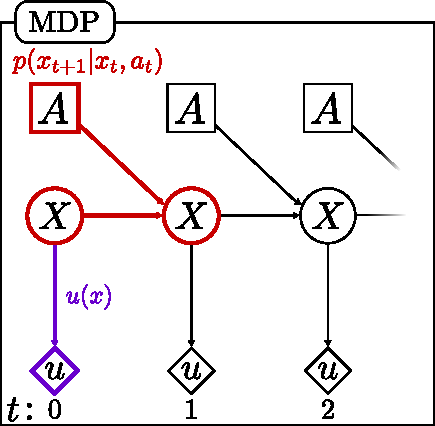
\includegraphics[width=0.45\textwidth]{/home/guillaume/Documents/Thesis/ch2-Background/Figures/mdp3.pdf}}
  \subfigure[on-policy]{\label{fig:mdp_on}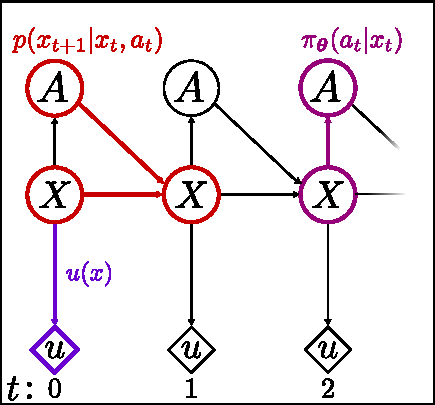
\includegraphics[width=0.45\textwidth]{/home/guillaume/Documents/Thesis/ch2-Background/Figures/mdp2.pdf}} 
  \caption{Dynamical Bayesian Network of a Markov Decision Process; it encodes the temporal relation between the random variables (circles),
  utilities (diamond) and decisions (squares). The arrows specify conditional distributions. In \textbf{(a)} the decision nodes are not considered 
  random variables whilst in \textbf{(b)} they are. From these two DBN  we can read off two conditional distributions, the state transition distribution (in red) and the action distribution (in purple). }
    \label{fig:mdp}
\end{figure}

Solving a MDP means finding a policy whose actions in any given state will always maximise the expected utility. Such 
a policy is usually denoted as $\pi^*$, the \textbf{optimal policy}. As in decision theory, the expected utility is the utility 
of  a sequence of states $u(x_{0:T})$ weighted by its probability. The graphical representation (Figure \ref{fig:mdp} (a)) allows 
the probability of a sequence of states and actions, to be read off directly: 
\begin{align}\label{eq:joint_state_actions}
  p(x_{0:T},a_{0:T-1}) &= p(x_{0}) \prod_{t=0}^{T-1} p(x_{t+1}|x_t,a_t) \\
  u(x_{0:T}) 	       &= u(x_0) + \gamma u(x_1) + \dots + \gamma^{T-1} u(x_{T-1})  + \gamma^T u(x_T)
\end{align}
We are interested in finding the sequence of actions, $a_{0:T}$, which will maximise the expected utility function:
\begin{equation}\label{eq:temporal_expected_utility}
 \argmax_{a_{0:T-1}} U(x_{0:T},a_{0:T-1}) = \max_{a_0} \sum\limits_{x_1}   \cdots  \max_{a_{T-1}} \sum\limits_{x_T} \Bigg( p(x_{0:T},a_{0:T-1}) u(x_{0:T}) \Bigg)
\end{equation}
Solving the above directly in its current form would to lead to an exponential complexity. Making use of the first order 
Markov assumption and that current utilities do not depend on future utilities, the summations can be re-arranged and 
a recursive pattern emerges which can be exploited: %which results in Equation \ref{eq:expansion}
\begin{align}\label{eq:expansion}
 &\argmax_{a_{0:T-1}} U(x_{0:T},a_{0:T-1}) =\max_{a_0} \sum\limits_{x_1}   \cdots  \max_{a_{T-2}} \sum\limits_{x_{T-1}} p(x_{0:T-1},a_{0:T-2})  \nonumber\\
 &\left( u(x_{0:T-2}) + \gamma^{T-1} \left( u(x_{T-1}) +  \gamma \max_{a_{T-1}} \sum\limits_{x_{T}} p(x_{T}|x_{T-1},a_{T-1}) u(x_{T}) \right) \right)
\end{align}
From the rearrangement we notice that Equation \ref{eq:expansion} has the same functional form as Equation \ref{eq:temporal_expected_utility}, 
except that the recursive component can be summarised by Equation \ref{eq:bellman}, which is known as 
the \textbf{Bellman} optimal equation (the asterisk indicating that it is optimal),
\begin{equation}\label{eq:bellman}
 V^*(x_t) := u(x_t) + \gamma \max_{a_t} \sum\limits_{x_{t+1}} p(x_{t+1}|x_t,a_t) V(x_{t+1})
\end{equation}
where for the terminal state $V_T(x_T) = u(x_T)$. The Bellman equation is a means of solving a sequential decision problem 
through use of dynamic programming. It shows that the utility of the current state is based on the immediate utility and 
the discounted maximum utility of the next state. Making use of this recursion reduces the computation complexity which is now 
quadratic in the number of states, $\BigO(T\, |A|\, |X|^2)$. To find the optimal value and subsequent policy an approach 
would be to repeatedly apply the Bellman equation to each state until the value function converges. What makes the problem 
difficult to solve is maximisation over the actions. This induces two problems, the first is that the optimisation is nonlinear 
and the second is that if the action space is continuous the maximisation will be expensive to compute.
This brings into play the two main approaches to solving a MDP: \textbf{off-policy} and \textbf{on-policy}.
Off-policy methods solve directly for the optimal value function, $V^*(x)$, and perform the maximisation over the actions. \textbf{Value-Iteration (VI)}
is such a method. On-policy approaches, $V^{\pi}(x)$, find the optimal value and policy through repeating \textbf{policy evaluation} and
\textbf{improvement} steps. In the policy evaluation the value or utility of a policy is found through solving the on-policy version of the Bellman 
equation:
\begin{equation}\label{eq:on_policy_bellman}
  V^{\pi}(x_t) := u(x_t) + \gamma \sum\limits_{a_t} \policy(a_t|x_t) \sum\limits_{x_{t+1}} p(x_{t+1}|x_t,a_t) V(x_{t+1})
\end{equation}
In the policy improvement step, the policy is made more greedy by maximising the value function. Through the repetition of these two 
steps both the value function and policy converge to the optimal. On-policy methods are preferred in settings where the action 
space is highly continuous, such as in robotics. Using dynamic programming is however not the method of choice since it requires 
multiple passes through the entire state space and for this reason it is necessary to have the model of the state transition a priori. 
Instead \textbf{Reinforcement Learning (RL)} methods are used to find an optimal value and policy. RL is a sample based approach
in which an agent interacts with the environment gathering examples of state transitions and the utility and uses them 
to gradually solve the Bellman equation.

We introduced the formulation of a sequential decision process for the MDP model and showed how an optimal policy 
and value function are obtained through maximising the expected utility. The re-arrangement of the summations, known as
variable elimination, allows to exploits a recursive structure present in the Markov chain. The recursive component 
turns out to be the Bellman optimal equation, which when solved (via dynamic programming or reinforcement learning) results 
in an optimal value and policy function. A MDP models the uncertainty inherent in the state transition but not the uncertainty 
of the state. The MDP assumes that the state space is always fully observable, which is a strong assumption. In robotics, the 
on board sensors return an estimate of the state with a certain amount of uncertainty associated with it. To take this additional
uncertainty into consideration the MDP has to accommodate it. This leads to a Partially Observable Markov Decision Process (POMDP).





% Define box and box title style
\tikzstyle{white_box}  = [draw=black, fill=white, very thick,  rectangle, rounded corners, inner sep=10pt, inner ysep=20pt]
\tikzstyle{fancytitle} = [fill=white,draw= black, text=white,rounded corners=1mm,text=black]


\subsection{POMDP}
%\begin{equation}
% y_t =  \begin{bmatrix}
%       r    \\
%       \phi \\
%     \end{bmatrix} \in \mathbb{R}^2
%\end{equation}

A POMDP is a popular approach for formulating a sequential decision process in which both motion and observation 
uncertainty are considered. In this partially observable setting the agent does not know with exactitude the state of the environment,
but is able to observe it through his \textbf{sensors}. We define a sensor mathematically as being a function of the 
state space, $x_t$, relating to an observation, $y_t$, corrupted by some noise, $\epsilon_t$,

\begin{equation}\label{eq:sensor}
  y_t = h(x_t) + \epsilon_t
\end{equation}

The sensor function $h(x_t)$ can be linear or non-linear and the additive noise term $\epsilon_t$ can 
be Gaussian (usually the case), non-Gaussian, state dependent or not. The uncertainty of the latent state, $x_t$, is quantified by a probability distribution, $p(x)$. 
This probability distribution represents all the hypothetical positions in the world in which the agent can be found. In Figure \ref{fig:belief_update_example} \textbf{(a)} an agent is located in a square yard 
containing a wall. Initially the agent is confident of his position; his state uncertainty $p(x_0)$ is low, represented 
by the blue probability density. However during a circular displacement the agent skids and the state uncertainty is increased 
by the state transition function, $p(x_{t+1}|x_t,a_t)$; this step is referred to as \textbf{motion update}. To reduce the uncertainty, the agent takes a measurement, $y_t$, with 
his sensors which provide range, $r$, and bearing, $\phi$, information with respect to the wall, see Figure \ref{fig:belief_update_example} \textbf{(b)}.
The agent uses the model of his sensor, known a priori, to deduce all possible locations in the world from where the current 
measurement could have originated. This model is known as the measurement likelihood function: 
\begin{equation}\label{eq:likelihood}
 p(y_t|x_t) = \mathcal{N}(y_t - h(x_t);0,\Sigma)
\end{equation}
The measurement likelihood function makes use of the measurement function $h(x)$ and it models the noise 
in the sensor. In this case the noise model, $\epsilon_t$, is Gaussian, paramaterized with mean zero and covariance $\Sigma$.
Typically the parameters of the measurement likelihood function are learned a priori.

\begin{figure}
  \centering
  \subfigure[]{\label{fig:motion_update}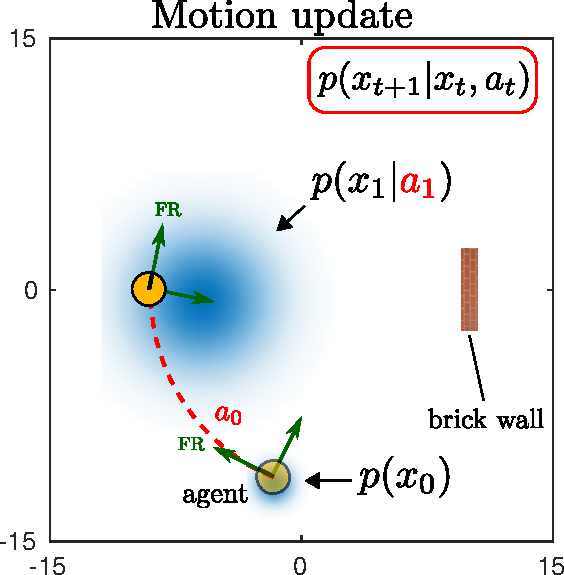
\includegraphics[width=0.45\textwidth]{/home/guillaume/Documents/Thesis/ch2-Background/Figures/motion_update.pdf}}
  \subfigure[]{\label{fig:measurement}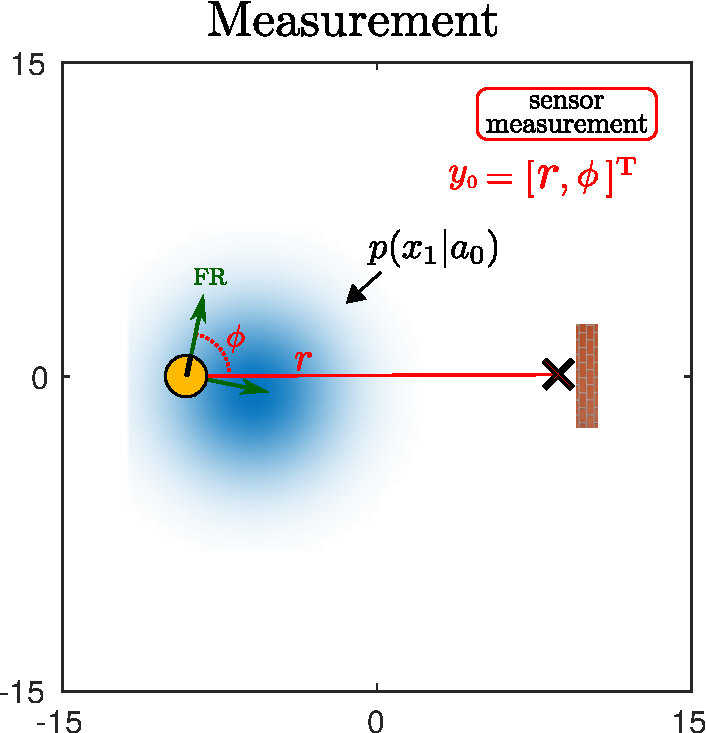
\includegraphics[width=0.45\textwidth]{/home/guillaume/Documents/Thesis/ch2-Background/Figures/measurement.pdf}} 
  \subfigure[]{\label{fig:likelihood}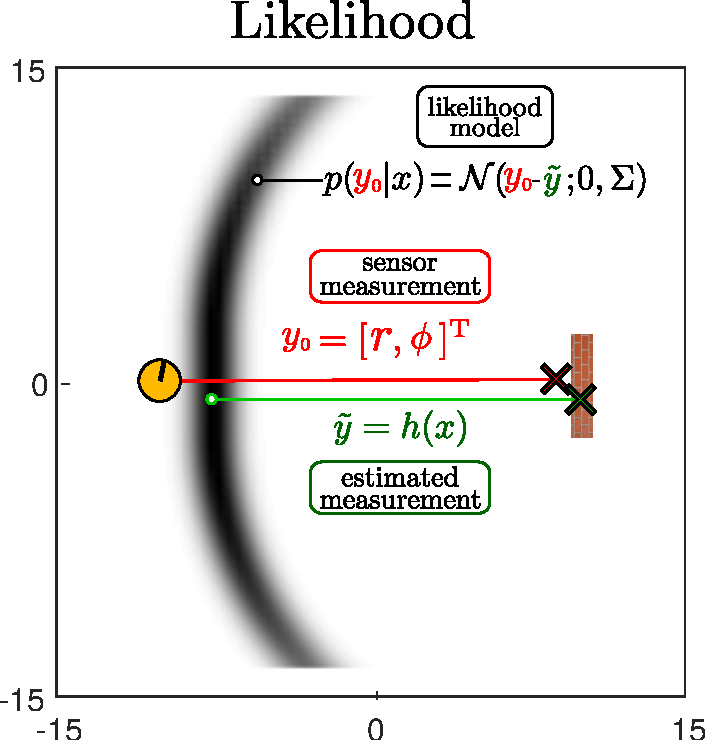
\includegraphics[width=0.45\textwidth]{/home/guillaume/Documents/Thesis/ch2-Background/Figures/likelihood.pdf}} 
  \subfigure[]{\label{fig:measurement_update}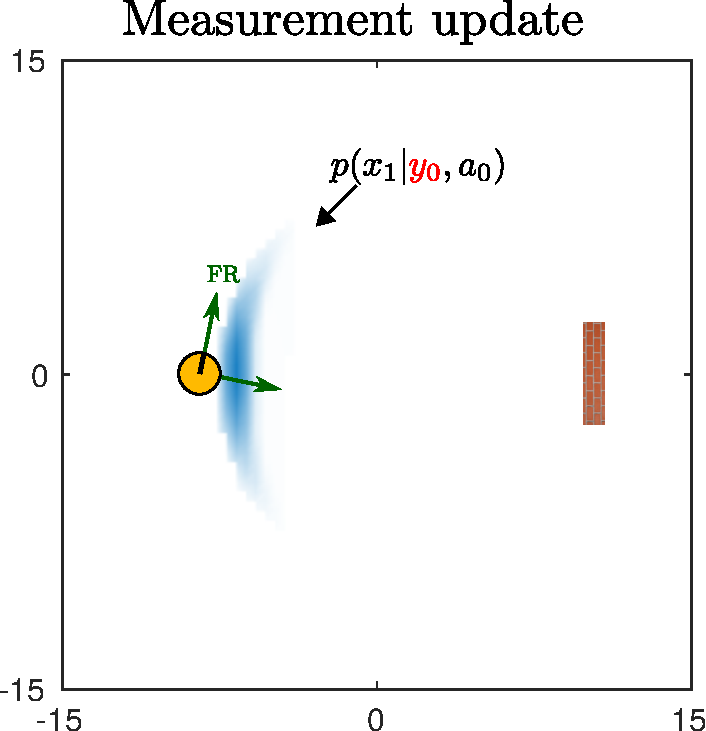
\includegraphics[width=0.45\textwidth]{/home/guillaume/Documents/Thesis/ch2-Background/Figures/measurement_update.pdf}} 
 \caption{\textbf{(a)} An agent is located to the south west of a brick wall. It is equipped with a 
  range sensor. The agent takes a forward action but skids, which results in a high increase of the uncertainty.\textbf{(b)} 
  The agent takes a measurement, $y_0$, of this distance to the wall; because his sensor is noisy his estimate is inaccurate. 
  \textbf{(c)} The agent uses his measurement model to evaluate the plausibility of all locations in the world which would result in a similar
  measurement; illustrated by the likelihood function $p(y_0|x_0)$. \textbf{(d)} The likelihood is integrated into the probability 
  density function; $p(x_0|y_0) \propto p(y_0|x)p(x_0)$.}
  \label{fig:belief_update_example}
\end{figure}

In Figure \ref{fig:belief_update_example} \textbf{(c)} the likelihood is illustrated. The dark regions indicate areas of high 
likelihood, which are possible locations from which the sensor measurement could have originated. The value of the measurement
likelihood function is then integrated into the state space probability density function; this step is referred to as \textbf{measurement update}.

The two update steps, motion and measurement, are part of a recursive state estimation process called a \textbf{Bayesian state space filter}, 
which we formalise below in Equation \ref{eq:motion_update}-\ref{eq:measurement_update}.
\begin{figure}
\centering
\begin{tikzpicture}
\node [white_box] (box){%
     \begin{minipage}{0.9\textwidth}
     The Bayesian filter turns a prior probability distribution over the state space, $p(x_t|y_{0:t-1},a_{0:t-1})$,
  to a posterior $p(x_t|y_{0:t},a_{0:t})$ by incorporating both motion and measurement. Applied recursively it 
  keep a probability distribution over the state space which considers all the past history of actions and observations. We define 
  the application of these two steps by the filter function $\tau$, which takes the current belief, the applied action 
  and measurement, and outputs the next belief, $b_{t+1}$.\\
  
  \textbf{Motion update}
	\begin{equation}\label{eq:motion_update}
	  p(x_t|y_{0:t-1},a_{0:t}) = \int p(x_t|x_{t-1},a_{t-1})\, p(x_t|y_{0:t-1},a_{0:t-1})\;da_{t-1}
	\end{equation}
      \textbf{Measurement update}
	\begin{align}\label{eq:measurement_update}
	  p(x_t|y_{0:t},a_{0:t})   &= \frac{1}{p(y_t|y_{0:t-1},a_{0:t})}p(y_t|x_t)\,p(x_t|y_{0:t-1},a_{0:t}) \\
	  p(y_t|y_{0:t-1},a_{0:t}) &= \int p(y_t|x_t)\,p(x_t|y_{0:t-1},a_{0:t}) dx_t
	\end{align}   
	\textbf{Filter function}\\
	\begin{equation}
	  b_{t+1} := \tau(b_t,a_t,y_t) 
	\end{equation}
    \end{minipage}
};
\node[fancytitle, right=10pt] at (box.north west) {Bayesian filter};
\end{tikzpicture}%
\caption{Bayesian state space filter.}
\end{figure}

The motion model, Equation \ref{eq:motion_update}, updates the position of the probability distribution according to 
the applied action, $a_t$, and adds uncertainty by increasing the spread of the distribution. The measurement information is 
then incorporated by Equation \ref{eq:measurement_update}. The measurement likelihood always reduces the uncertainty 
or leaves it constant. The Bayesian state space filter is such an important 
component to belief space decision making that we define it by the filter function, $\tau(b_t,a_t,y_t)$, which 
takes as input the current belief, applied action and sensed measurement and returns the resulting belief $b_{t+1}$.
The state space filter is an essential component to a POMDP which will become apparent later.

%Depending on the type of sensors: stereo cameras, infra red sensors, Kinect, 
%omnidirectional camera, etc.., there is uncertainty associated with it. It is thus important 
With the latent state, its relation to the observation variable and the Bayesian filter defined, we can introduce the POMDP model
in Figure \ref{fig:pomdp} (\textit{left}). It has the same Markov chain structure as the MDP, introduced in the previous section, but the state space $X$ is latent and 
a new layer of observation variables $Y$ is added. 

\begin{figure}
 \centering
  \centering
  \subfigure[]{\label{fig:sub_pomdp}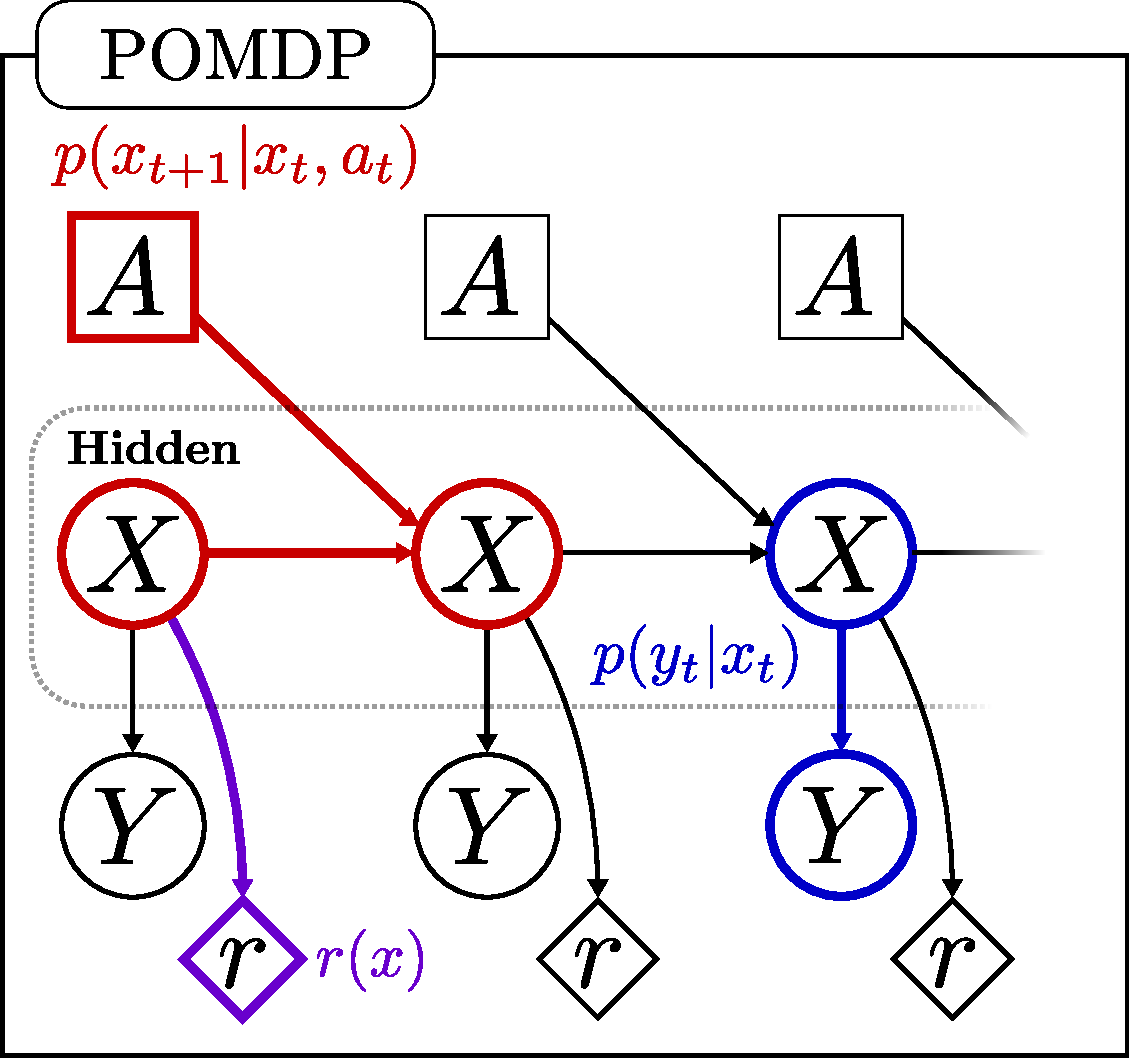
\includegraphics[width=0.45\textwidth]{/home/guillaume/Documents/Thesis/ch2-Background/Figures/pomdp2.pdf}}
  \subfigure[]{\label{fig:sub_bmdp}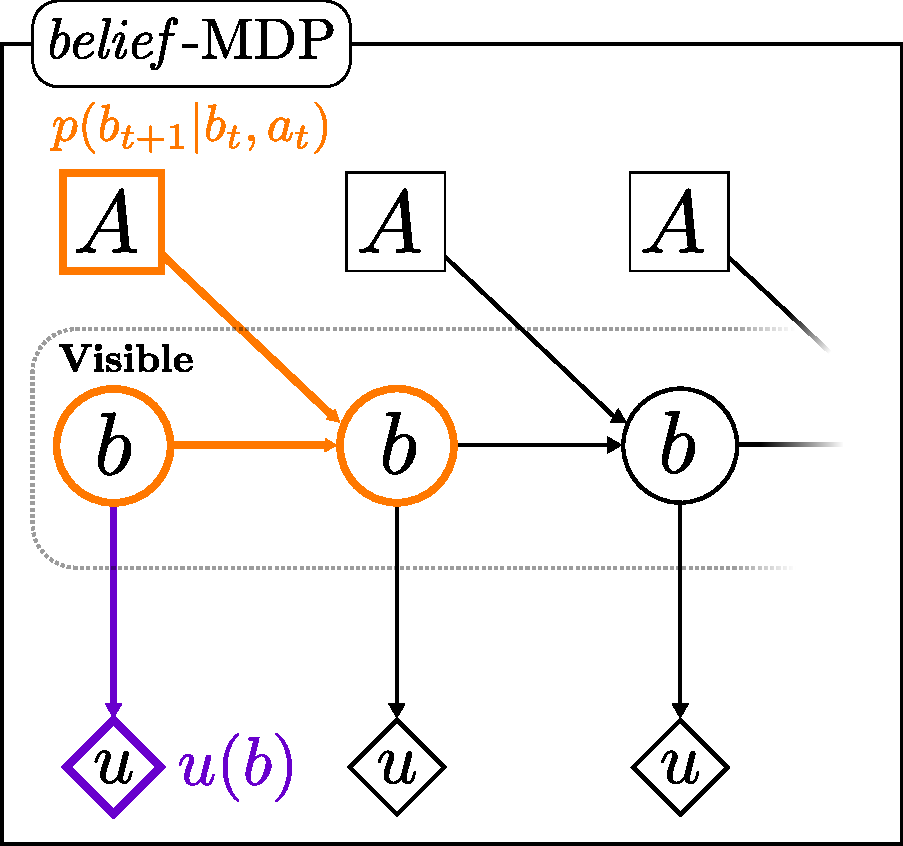
\includegraphics[width=0.45\textwidth]{/home/guillaume/Documents/Thesis/ch2-Background/Figures/pomdp3.pdf}} 
  \caption{\textbf{(a)} POMDP graphical model. The state space, $X$, is hidden, but is still partially observable through a 
  measurement, $Y$. \textbf{(b)} The POMDP is cast into a belief Markov Decision Process, belief-MDP. The state space is 
  a probability distribution, $b(x_t) = p(x_t)$, (known as a belief state) and is no longer considered a latent state. The original state 
  transition function $p(x_{t+1}|x_t,a_t)$ is replaced by a belief state transition, $p(b_{t+1}|b_t,a_t)$. The reward 
  is now a function of the belief.}
  \label{fig:pomdp}
\end{figure}

%We will see that because the state space is hidden it will cause complications to the maximisation of the expected utility.
%Since the states are not observable, the agent cannot choose its actions based on the state. The explicit 
%representation of the past events is typically memory expensive. Instead it is possible to summarize all relevant %
%information from previous actions and observations in a probability distribution over the state space, known as the
%belief state. 

As the state space is only partially observable the expected utility has to be computed for each possible history of states, actions and observations.
All approaches in the literature instead encapsulate all these possible histories into a belief state $b(x_t)$ (for short notation $b_t$)
which is a probability distribution (also referred to as an information state, \textit{I}-state) over the state 
space $x_t$ and use this new state description to cast the POMDP into a \textbf{belief-MDP} (states are probability distributions, 
beliefs). By casting a POMDP into a \textit{belief}-MDP the state space is considered observable and we recover the same structure 
as in the standard MDP problem.

As we are working within a belief space the reward function has to be adapted to:
\begin{equation}
  u(b_t) = \sum_{x_t} u(x_t)\, b(x_t) = \mathbb{E}_{b_t}\{u(x_t)\}
\end{equation}
which is an expectation. The goal as before is to find a sequence of actions 
which will maximise the expected utility. Since our \textit{belief}-MDP has the same structural form as the MDP, the solution 
to the problem is the same Bellman equation derived previously. We just substitute the new belief transition function 
and we get the corresponding belief Bellman Equation, \ref{eq:belief_bellman}.
\begin{equation}\label{eq:belief_bellman}
 V^*(b_t) = u(b_t) + \gamma \max_{a_t} \sum_{b_{t+1}} p(b_{t+1}|b_t,a_t)\,V^*(b_{t+1})
\end{equation}
However, using this equation in this form is problematic, as we are summing over the space of beliefs (which is high dimensional 
and infinite for the continuous case) and the transition function is a probability distribution over beliefs. 
The key to overcome this problem is to realise that if we know what the current measurement and applied action are, 
there is only one valid possible belief, $b_{t+1}$, and
the summation over beliefs vanishes. This can be seen by substituting the belief transition function,
Equation \ref{eq:belief_state_transformation}, into the Bellman equation Equation \ref{eq:belief_bellman}.
\begin{equation}\label{eq:belief_state_transformation}
 p(b_{t+1}|b_t,a_t) = \sum_{y_t} p(b_{t+1}|b_t,a_t,y_t)\,p(y_t|y_{0:t-1},a_{0:t})
\end{equation}
After the substitution and re-arrangement of the summation we get Equation \ref{eq:max_component}. 
Since the observation is known (because the outer summation is over $y_t$), the summation over the beliefs vanishes since there is only one possible future belief which is given by the 
Bayesian filter function $b_{t+1} = \tau(b_t,a_t,y_t)$,
\begin{equation}\label{eq:max_component}
u(b_t) + \gamma \max_{a_t} \sum_{y_t} \underbrace{\left( \sum_{b_{t+1}} p(b_{t+1}|b_t,a_t,y_t)\,V^*(b_{t+1})\right)}_{1 \cdot V^*(\tau(b_t,a_t,y_t))}\, p(y_t|y_{0:t-1},a_{0:t})
\end{equation}
which simplifies to:
\begin{align}\label{eq:final_belief_bellman}
  V^*(b_t) &= u(b_t) + \gamma \max_{a_t} \sum_{y_t}  p(y_t|y_{0:t-1},a_{0:t}) \,V^*(\tau(b_t,a_t,y_t))\nonumber  \\ 
	   &= u(b_t) + \gamma \max_{a_t} \displaystyle \mathop{\mathbb{E}}_{y_t}\{V^*(b_{t+1})\}
\end{align}

The belief Bellman equation is intuitive. The value of the current belief is the immediate utility plus the value of the 
future belief states weighted by the probability of a measurement which would result in these future belief states. 
An exact solution exists only when considering a finite state, action and observation space and a finite planning horizon $T$, \cite{Sondik_1973}.
The belief-MDP can be solved with value iteration but each backup operation (application of the bellman equation) 
results in an exponential growth in the number of parameters needed to represent the value function, which 
is computationally intractable.

Most early techniques for solving POMDPs used value iteration. The preference for persisting in doing this, given the computational
burden, is that since the utility function uses a linear operator (the expectation) and that the Bellman backup operation 
(applying the Bellman equation to the current value function) preservers the linearity, the value function after each 
updates is Piece Wise Linear and Convex (PWLC). A good text on the implementation of exact value iteration for POMDPs can be 
found in \cite[Chap. 15]{Thrun_2005} and \cite{Kaelbling_1998}.

In summary there are two problems in solving a POMDP:
\begin{itemize}
 \item \textbf{curse of dimensionality}: A discrete state space of size $N$ will result in a belief space of dimension $N-1$. The discretization
 choice will greatly impact the computational cost of Value Iteration.
 \item \textbf{curse of history}: The space and computational complexity in the worst case is exponential with respect to the planning 
 horizon, $T$, \cite{POMDP_approach_2010}.
\end{itemize}

Given such complexity it is hard to see POMDPs being actually usable for real world scenarios. As a result many approximate 
techniques have emerged with some being very successful. In the next section, we survey the literature 
and the developments of approximate POMDP algorithms and their applications.

P-SPACE \cite{psace_mdp_1987} complete

%Before this point and before only value iteration on this subset instead of considering all beliefs.  If you have a $10 \times 10$ gird, this results in a total of a $100$ states %and a belief state of a $100$ dimensions! The PBVI approach initiated a renewed effort in 
%porting VI to POMDPs with larger and larger state spaces

%It turns out that computing a value function using the above bellman function is not computationally tractable.

%Solving 
%a POMDP problem as for the MDP case consists of finding the optimal value function from which the optimal policy can 
%b%e derived. Essentially the same dynamic programming and reinforcement learning techniques can be applied to solve 

%From considering the decision belief tree of the POMDP, Figure \ref{fig:pomdp_bel_tree}, we can appreciate the complexity of the problem
%of finding an optimal policy. Given a discrete set of actions and observations to update the belief $b_1$ we have to consider a time 
%complexity of $\mathcal{O}(|U||Y|^T)$ where $T$ is the depth of the tree (the planning horizon). Given that we have a finite set of 
%belief the complexity solving the POMDP is $\mathcal{O}(|\mathcal{B}||U||Y|^T)$. 

% In the worst cast, the exact value update procedure could require time doubly exponential in the planning horizon, T.
%Why is POMDP so good: combine information gathering and goal directed actions in one. Give taxonomy of planning under uncertainty here.

\section{Literature review}\label{sec:lit_rev}

We review the latest methods of solving sequential decision problems under uncertainty. 
This is an extremely dense and spread out area of research, no doubt because of its 
importance. If uncertainty is not considered adequately, the control policy 
risks being suboptimal or lead to drastic failure. 


\begin{figure} 
\centering
\hspace*{-4cm}
\begin{minipage}{\linewidth}
\begin{tikzpicture}[every annotation/.style = {draw, fill = white, font = \Large}]

\path[mindmap,concept color=black!40,text=white, every node/.style={concept,circular drop shadow},  
    root/.style    = {concept color=black!40,font=\Large\bfseries},
    level 1 concept/.append style={level distance=15em,sibling angle=90,font=\large\bfseries},
    level 2 concept/.append style={level distance=9em,font=\bfseries},
  ]
    node[root] at (0,0)  {Acting under uncertainty}[clockwise from=135]
    child [concept color=red!90]  { node [concept] (PolicySearch) {Policy search} [clockwise from=180]
          child { node (EM) {EM} }
	  child { node (Gradient) {Gradient} }
	  child { node (GradientFree) {Gradient free}
        }
    }
    child [concept color=teal!90] { node {Planning}[clockwise from=50]
        child { node (BRM) {Belief\\ road maps}}
        child { node (OptimalControl) {Optimal control}}
    }
    child [concept color=orange!90] { node {Heuristics}[clockwise from=-10]
        child { node {Info.\\Gain}}
        child { node {QMDP}}
        child { node {Myopic}}
    }
    child [concept color=blue!90] { node  [concept] (ValueIteration) {Value Iteration}  [clockwise from=-55]
	child { node (Latent) {Latent\\ VI}}
        child { node (ApproxVI) {Approx. VI}}
        child { node (PBVI) {Point-base\\ VI}
        }
    };
    
    \begin{scope}[mindmap]
      \node[fill={green!40!black},circle,level 1,color=green!40!black,text=white,font=\large\bfseries] (ActorCritic) at (-5,0) {Actor-critic};
    \end{scope}
  
    \path (ActorCritic) to[circle connection bar switch color=from (green!40!black) to (blue!90)] (ValueIteration) ;
    \path (ActorCritic) to[circle connection bar switch color=from (green!40!black) to (red!90)] (PolicySearch) ;
  
    \info[7]{Latent.south}{below,anchor=north}{
      \item E-PCA
    }
    
    \info[9]{ApproxVI.south}{below,anchor=north}{
      \item MC-POMDP
    }
    
    \info[9]{PBVI.south west}{below,anchor=north}{
      \item SARSOP
      \item HSVI2
    }
  
    \info[7]{EM.south west}{below,anchor=north}{
      \item PoWER
    }
  
    \info[10]{Gradient.north west}{above,anchor=north,yshift=1cm}{
      \item REINFORCE
    }

    \info[6]{ActorCritic.south west}{below,anchor=south,xshift=-1.5cm,yshift=0.5cm}{
      \item eNAC
    }
    
    \info[9]{OptimalControl.south}{below,anchor=north}{
      \item B-LQR
      \item LQG-MP
    }
    
    \info[9]{BRM.north}{below,anchor=north,yshift=1.3cm}{
      \item BRM
      \item FIRM
    }
\end{tikzpicture}
\end{minipage}
\caption{Mind-map of AI and robotic methods for acting under uncertainty.}
\end{figure}
	
% Vision and range sensors can estimate the pose of an object, but there is still residual uncertainty.
% Tactile sensing, combined with proprioception, can give highly reliable inforation about object position.
% Uncertainty due to sensor noise is particularly problematic for fine manipulation tasks[1], such as grasping 
% and pushing a small button on a drill, hookoing the figuers of a hand around a small button on a drill.

\subsection{Value Iteration}\label{lit:VI}

The POMDP formulation introduced previously is the main theoretical starting point of policies which
consider uncertainty optimally. However solving an exact POMDP through dynamic programming (value iteration) is 
computationally intractable and an exact solution only exists for discrete state, action and observation space \cite[Chap. 15]{Thrun_2005}. 
This intractability, in which only problems with a few states could be solved has inhibited the application of the POMDP framework to robotics. 

\subsubsection{Point-base Value Iteration}

The first breakthrough of the application of VI in belief space to a robotic application was Point-Base Value Iteration (PBVI) \cite{PBVI}. It allowed VI to be applied to a robotic 
navigation problem consisting of 626 states in a hospital patient search task. The key insight to scale VI was to only consider a subset of belief 
states which were reachable and relevant to the problem. This is achieved by smart sampling techniques and only performing VI backups on beliefs states which are relevant. 
From this point most research has focused on determining efficient strategies to sample belief points and on which to apply VI. Heuristic Search Value Iteration (HSVI1) (\cite{HSV}) 
and HSVI2 (\cite{HSVI2}) use forward search heuristics to find relevant beliefs by keeping a lower and upper bound on the current estimated value function. The belief tree 
is expanded by choosing an action and observation with relation to the potential future effect on the value of the bounds, which are being minimised. HSVI has a comparable performance with respect to classical PBVI except in the
game of tag (a benchmark problem), in which it fairs significantly better. 
A method developed after HSVI, named Forward Search Value Iteration (FSVI) (\cite{FSVI}) takes an alternative approach to keeping an upper and lower bound on the 
value function, as in HSVI, since doing so results in a drastic increase in the computation time necessary to find a solution. Instead FSVI assumes that the state 
space is fully observable and first solves the MDP for this case. The MDP is then used to generate a set of belief points for the PBVI solver. This is achieved by 
taking the Most Likely State (MLS) and to follow the MDP policy accordingly. It is orders of magnitude faster than HSVI and results in comparable polices. FSVI fairs badly however when information gathering actions are necessary. 
Since it is essentially using a myopic policy to generate its samples, these will be insufficient to find the global optimal policy when the solution requires information gathering actions. The very last sampling generation technique to date, which is considered to be the most efficient, is SARSOP (\cite{SARSOP}).
It uses aspects from both HSVI and FSVI. It keeps upper and lower bounds on the value function and also uses the MDP solution to generate samples. 
The key idea of SARSOP is to sample belief points which will contain the optimal set of samples necessary to achieve an optimal policy.  
Both SARSOP and HSVI2 are considered state of the art in PBVI value approximation techniques. See \cite{POMDP_approach_2010} for a review and comparison of both techniques on problems 
with thousands of states including simulation examples in grasping, tracking and UAV navigation. 

These methods are well suited to addressing problems which are easily expressed in a discrete state space. All considered problems are simulation based and 
no physical interaction problems are considered. Besides the belief set generation problem, interest has also been poised on porting the PBVI to a continuous state space.
An example of a continuous action space PBVI method is Perseus \cite{Spaan05icra}, in which the authors replace the maximisation over the action by sampling the actions from a 
parametric continuous representation. In \cite{PBVI_C_2006} the state space, transition and observation model are represented by Gaussian Mixtures and the authors consider a particle set or Gaussian mixture representation of the belief. 
The authors show that a continuous representation of the state space preserves the PWLC property of the value function. They extend their method to continuous action and observations 
through sampling instead of discretising. Results are shown in a 1D continuous corridor setting. In a 
more recent approach \cite{solving_continous_pomdps_2013} a discrete state presentation of a continuous state space is learned and is combined with sampling
techniques to solve the continuous integrals present in the Bellman equation. The explicit learning of the state representation leads to an increased performance
when compared to the other continuous state PBVI methods. 

PBVI techniques have come fare since their first application to robotic navigation back in 2003 and have lead to a rapid increase of interest. 
Initially only a few hundred states could be considered and now problems with over tens of thousand of states are being solved in seconds (very problem specific of course). 
Most of the research has focused on how to gather a good set of sample beliefs efficiently. Later efforts focused on adapting PBVI 
to continuous state spaces more suited to robotic applications. The main approach consists of using sampling techniques to overcome 
the maximisation over the actions (when considering continuous actions) or to choose a suitable parametric representation of the transition, observation 
and utility model so that the Bellman equation can be solved in closed form. Most evaluations of have focused on simulated and simplified robotic 
navigation problems in 1D and 2D. We have not discussed online POMDP-solvers since they are also based on VI and sampling techniques and thus share 
a lot of similarities with PBVI. We refer the reader to \cite{Ross08onlineplanning} for a detailed review. In summary, trying to preserver the PWLC property 
of the value functions leads to complicated VI methods which are difficult to port to fully continuous state, action and observation space. Efforts which 
have attempted to do this have not yet be shown to scale. As a result of this difficulty, of making this transition to a fully continuous space, approximate value 
iteration methods have been explored as an alternative. In approximate value iteration the PWLC property of the value function is dropped and is 
represented by a regression function.

%		\cite{MCVI_CS_POMDPs}	% sampling techniques 
% PBVI methods: \cite{Veiga14aaai} 	% Pedro Lima Point-Based method for Factor value 

\subsubsection{Approximate Value Iteration}

Point-based Value Iteration techniques try to preserve the PWLC property of the value function. This directly 
leads to a discretization of the state space which if continuous by nature, is prone to the curse of dimensionality.
An alternative approach is to represent the value function by a non-parametric function, parameterize the belief space and perform approximate 
dynamic programming.  

%An alternative approach is to represent the belief space by a parametric representation, for instance as a Gaussian function. 
%The value function is then defined as a function of the parameters of the Gaussian. This approach in effect greatly 
%diminishes the dimensionality problem but does away with the PWLC property of the value function. Instead to generalise 
%the value of particular parameter a regressor function is needed and to learn it approximate dynamic programming techniques 
%are used.

A very first successful example of this approach is Monte Carlo POMDP (MC-POMDP) \cite{MC-POMDP} in which a continuous 
state, action and observation version of the Heaven \& Hell benchmark problem was solved successfully with a working 
implementation on a non-simulated mobile base.  
The belief was represented by a particle filter and the policy by a Q-value function, whose functional form was 
a non-parametric regressor (k-nearest neighbour) of the particle filter. The distance metric was the sample KL divergence
between two particle sets. The POMDP was solved through Reinforcement Learning (interaction with the environment) and 
approximated dynamic programming also known as experience replay, batch RL or Fitted Q-Iteration (FQI) \cite{Tree_batch_2005}. 
Although highly computationally demanding the method was successful. 

This inspired many similar approaches such as \cite{mc_update_ppomdps} where the belief state filter was an 
Extended Kalman Filter (EKF), the value function was also non-parametric and the POMDP was solved via FQI. 
When compared with Perseus in a discretized 2D localisation task both approaches reached equivalent 
policies but the authors method achieved it far faster than Perseus, a PBVI method. 

% 2) A very large state space and do away with 
An alternative approach is to represented the history of the previous states or observations in an augmented state space and the treat the problem 
as a standard MDP. In this way the partial observability is directly encoded in the state representation. The motivation is that in contrast to 
POMDPs there has been fare more research focused on MDPs and much work has been done on the application of non-linear function 
approximators for representing the value function in combination with reinforcement learning optimisation techniques to solving them.
A successful example was the usage of a multi-layer perceptron as a Q-value function approximator, Neural Fitted Q-Iteration (NFQ) \cite{neura_fqi_2005}.
This approach was successfully applied to the standard RL benchmarking problems (carte pole, acrobat, mountain care), but no partially observable
setting was considered. Later in \cite{DRQ_AAAI_2015} the authors applied a Deep Recurrent Q-Network (DRQN) (extension to the work in \cite{mnih-dqn-2015}) to capture the history of states 
in a game of Pong where the state space was occluded half the time. By introducing a long term memory component the POMDP in effect is turned into a MDP and the authors apply an optimisation approach similar to FQI. 

The advantage of these approaches is that problem with very large state spaces or continuous state spaces can be solved by using
standard machine learning function approximation methods. These methods are easier to understand and implement and adapting 
POMDP methods to them is relatively straight forward. This is one particular way of dealing with the curse of dimensionality but not the 
only way. An alternative is to find a latent belief space which is of a much lower dimension than the original and perform value iteration in 
that space.

\subsubsection{Latent Value Iteration}

% 1) Belief space compression and value iteratrion
Latent belief space or belief space compression is a way of addressing the curse of dimensionality. The assumption 
is that although the belief space is of considerable size (thousands of dimensions) a latent belief space exists 
which is considerable smaller in terms of dimensions (a dozen).
A first approach of compressing the belief is to transform it into a set of sufficient statistics (first and second moment for example) and  
treat the problem as a fully observable MDP in which the states are sufficient statistics of the beliefs. 
In \cite{Roy99coastalnavigation} the authors do just this, they compressed the filtered belief to its mean and entropy and performed VI on 
this augmented state space in a navigation task in which the goal was to reach a location with a minimum amount of uncertainty. This approach,
called Augmented MDP (AMDP), brings a great simplification to solving the POMDP but at the cost of a lossy belief compression. 

In further developments \cite{belief_compression_2005} compared both PCA and exponential-PCA (E-PCA) \cite{EPCA_2003}, as a means of belief compression technique
to find a low dimensional belief space. The authors showed that an original belief of thousands of dimensions could be compressed 
to a 10 dimensional belief space whilst retaining most of the information. This approach was shown to be superior to AMDP. It requires however 
computationally expensive transitions back and forth between the low and high dimensional belief states, a necessary step for the the application of VI. The latest work in this 
area is \cite{bs_compression_2010} which investigates the use of non-negative matrix factorisation in combination with k-means 
clustering as a way of compressing the belief. There method showed some improvement over the E-PCA approach but was only evaluated 
on discrete benchmark problems.


Belief compression as a means of reducing the curse of dimensionality is an interesting approach. The 
caveat is that it requires discretising the belief to a fixed grid, collecting many samples and learning an 
appropriate set of belief-basis eigenvectors. As such, the larger the state space, the larger the dimensionality and thus more
samples are required to find a suitable set of basis belief-eigenvectors. Surprisingly, belief space compression 
methods have not had wide attention although they shown promising results.


\subsubsection{Summary: Value Iteration}

Value Iteration seeks to find an optimal policy directly through applying the Bellman equation to a belief-MDP (POMDP)
and most of the research has focused on finding ways to alleviated the curse of dimensionality so that VI remains tractable 
in belief space. The first approach, PBVI, considers a relevant subset of the belief space. Because 
of the complexity involved in keeping the PWLC property of the value function which restricts its use in large state 
spaces, alternative approaches discard this property in favour of approximating the value function through machine learning
regression techniques. These approaches are considerably more simple to implement than PBVI solvers which require heuristic pruning 
techniques and are difficult to port to continuous state spaces in general. Alternative approaches have considered finding a latent
belief state and perform value iteration in this space. There has however been relatively little work in the latent belief space approach.

Overall, the above approaches consider mostly discrete actions even for the large state (history states) MDPs
which have been gaining recent attraction. There are only a few exceptions and these resort to sampling strategies 
or the usage of paramaterized high level actions. The next approach we consider addresses the problem of continuous
actions directly and are termed policy search methods.

\subsection{Policy search}\label{lit:policy_search}

The approaches seen so far use a value function to encode the problem. When the optimal value function is solved, a policy can be derived from it by taking an action which maximises the value function at each time step, a process known as making the policy greedy with respect to the value function. This requires learning a high dimensional value function of the belief space and the resulting policies are not necessarily 
smooth, as small changes in the value function can lead to drastic changes in the policy. Even small 
approximation errors in the value function can lead to very bad greedy policies \cite{gpomdp_2000}. 
There is no doubt that deriving a policy from a generic value function for highly continuous policy, such as in the case 
of controlling an articulated robotic arm, is not easy. 

This has lead to an alternate approach in which a policy is learned directly without a value function. An 
initial policy is defined in terms of a paramaterized function, $\policy$, and the utility is a function of the 
policy parameters, $u(\boldsymbol{\theta})$. The optimal policy is found by searching for the parameters $\boldsymbol{\theta}$ which 
will maximise the utility function. This is can be accomplished through various optimisation methods: gradient descent, gradient free, 
expectation-maximisation, etc...

% Policy Iteration
% Early work include the application of policy iteration to a finite state controller \cite{p_search_pomdp_1998}. A finite state controller
% is iteratively evaluated (VI) and then subsequently improved until an optimal policy is found. Evaluation of the policy is much faster 
% than solving the optimal bellman equation, since the maximisation over the actions is absent. 
% Reinforce (gradient based methods)
% Actor-critic methods (combine both value function and policy)
% REINFORCE - PoWER - PI2 - 
\subsubsection{Gradient: policy search}

A very early type of policy search was REINFORCE (likelihood ratio) algorithms
first introduced by \cite{reinforce_1992}. From a set of task executions, also called roll-outs, the gradient
of the utility function is estimated and used to improve the policy through gradient ascent. 
The key aspect of this approach is that the derivative of the cost function is independent of the state transition model 
and as a result the gradient can be estimated by Monte Carlo methods. Application of this methodology 
to a partially observable setting lead to Gradient POMDP, GPOMDP \cite{gpomdp_2000} in which the authors developed 
a conjugate stochastic gradient ascent algorithm to optimise a policy as a function of the current observations.
To be optimal, the whole history should be considered or some sort of memory (compressed history) should be introduced. 
In an extension to this method \cite{sis_pomdp_2002}, the authors used a HMM to represent the POMDP which they 
learned the parameters in conjunction with those of the policy. These are early examples of policy search approaches 
which are able to fair well on the early POMDP benchmark problems (Heaven \& Hell). 
The main difficulty is to reduce the bias and variance of the gradient estimate which preoccupies most gradient based approaches. 
Optimising the utility function via stochastic gradient ascent typically needs thousands of gradient estimates such that in expectation terms the parameters are maximising the cost function. 
An approach which mitigates this problem, coined Pegasus \cite{Pegasus_2000}, removes the stochasticity from the optimisation 
by setting the seed of the random number generator constant. A policy evaluation becomes deterministic and by repeating this process many times (different random seeds) the stochasticity
is present between the different evaluations and not within them. The end result is the same as stochastic gradient ascent 
(if repeated sufficient times) but is far easier to optimise individual non-stochastic problems. This policy search 
method was used to learn a set of controllers for a radio controlled helicopter \cite{heli_2004}, which is considered to 
be one of the very first successful applications of RL to a MDP/POMDP problem. Recent approaches to gradient based methods
include grasping objects under Gaussian position uncertainty \cite{dmp_iros_2011}, \cite{dmp_seq_2012}.

\subsubsection{Expectation-Maximisation: policy search}

One drawback of gradient based optimisation is that the learning rate  plays a significant role on the speed of convergence. 
An alternative approach consists of using Expectation-Maximisation (EM) methods \cite{PoWER_2009} which do not require a learning rate. Successful applications include: ball-in-a-cup, a humanoid learning the skill of archery \cite{archery_2010}, learning how to 
flip a pancake \cite{pancake_2010} and keeping balance on a two-wheeled robot \cite{Wang2016}. These are just some examples 
of the application of RL to continuous action and state space problems. When uncertainty is present, the maximum likelihood state estimate is typically taken 
and is treated as the true state. A good surveys on policy gradient search methods can be found in: \cite{p_search_surv_2011}, \cite{RL_robots_surv_2013}.

\subsubsection{Actor-critic: policy search}

Gradient and EM methods only optimise the parameters of the policy, also known as actor only methods. An alternative  
is to have a separate parameterization of the value and policy functions. This approach is known as an \textbf{Actor-Critic}, in which the gradient of the utility function is used both to update 
the value and policy functions. It has been shown that this approach reduces the variance of the gradient estimate and allows
to smoothly change the policy which is desirable when controlling a robot for instance, see \cite{ac_survey_2012} for a 
survey highlighting differences and advantages of policy search vs actor-critic methods. A successful application of actor-critic is (episodic) Natural Actor Critic (eNAC) \cite{eNAC_2003}, \cite{NAC_2008}, a method which uses the \textit{natural gradient} of the value function to update the parameters of a policy. The advantage of using the natural gradient is that it guarantees small changes in the distance between the successive roll-out trajectory distributions. Previous policy gradient methods did not have such guarantees, since small parameter changes of the policy could lead to large changes in the roll-out distributions, which is undesirable. In terms of performance NAC converges faster than GPOMDP and has been applied to learn Dynamic Motor Primitives (DMPs) to control a humanoid robot. 

\subsubsection{Summary: policy search}

For problems in which the state and action space are continuous, policy search is preferred to pure value iteration based methods, 
which is the case for articulated robotics. In this case, the policies are only guaranteed to be \textbf{locally optimal} as oppose 
to the VI methods which can find \textbf{global optimal} policies. However if the parameters of the policy are initialised 
such that it is in the vicinity of the global optimum of the utility function, then the local optimal will be global. 
A lot resides on the initialisation and dimensionality of the parameter space of the policy. 
In terms of using them to solve POMDPs, most examples, at least for robotic applications, act according to the Most Likely State (MLS) or 
are a function of a history of observations. In such a way the partial observability is \textbf{implicitly} encoded into the policy as 
opposed to explicitly as was the case for PBVI methods. 

Policy gradient methods are iterative and generally require a lot of data to be able to achieve a good policy. Also 
often the policies learned are not transferable between different tasks and have to be completely 
relearned. This of course depends on the representation of the state space which if task invariant causes no problem,
but unfortunately this is not the case. The next approach to treating uncertainty is more aligned with addressing this last issue 
of re-usability. These are the \textbf{planning} methods.

%In some applications your objective function might not be differentiable or the policy might be parameterised
%by a few parameters and approaches other than using a gradient exist. These methods are called gradient free and d

%dlicy search method
%In \cite{Martinez-Cantin2009}, finite horizon planning problem, belief dependent utility function. non-Gaussian, trades off exploration vs exploitation. The pomdp
%policy is represented by a parameterised path. Use PID controller to follow the planned path. Dynamic model is non-differentiable, cannot use gradient based optimisation methods.
%Use bayesian technique to approximate the cost function with a surrogate function that is cheaper to evaluate.
%sample parameters wit expected cost, learn a function relating parameter choice to cost. The parameterised policy trades off %exploration vs exploitation. Aim to 
%minimise the number of cost function evaluations. Minimise uncertainty about its pose (location and heading). Policy is %parameterised by a finite set of way points.	
%Same cost function as RL, but cost is with respect to the map (doing SLAM). Cannot use LQG to solve this problem 

\subsection{Planning}

Belief space planners leverage the power of traditional planning and optimal control techniques such as: A*, D*, RRT, Dijkstra and LQR to the belief state space. 
In most of the following techniques (with a few exceptions), a fundamental assumption made is that the motion and measurement models are Gaussian 
and as a result, a point in the belief space can be represented by the first and second moment: the mean and covariance. An important distinction with VI and Policy search methods is that planners
do not solve for a policy. These are online methods in the sense that they have to re-compute a set of 
actions at every time step as oppose to a policy which can directly query which action should be applied given the current state. 
The generic objective function used in belief space planning penalises for the amount of uncertainty at the goal and a cost is incurred 
for every step taken. The planned path will be a compromise between the exploitation actions, which seek to go directly to the goal, and information gathering actions, which seek to reduce the uncertainty.

\subsubsection{Belief space road maps}

An example of belief space planning is the application of Probabilist Road Maps (PMR) to a belief state space, \cite{BelRoadMap_2009}, referred to as Belief Road Maps (BRM). By taking advantage of the linear structure of the Kalman Filter update the authors show that the covariance matrix can be factorised such that a sequence of motion and measurement updates between two belief points in the BRM can be computed by a single linear operation parametrised by the current belief. 
The key advantage of this approach is that it allows for rapid replanning and is able to scale to large state spaces. 
The authors evaluated their planner in the MIT campus (simulated). Applications of this methodology include the control of an indoor 
quadrotor helicopter \cite{Quadrator_2008} and indoor navigation (\cite{FIRM_2011}, \cite{rob_online_bs_icra_2014}) 
(based on Feedback-based Information Road Maps FIRM , a similar approach in spirit to BRM).

\subsubsection{Optimal control}

Another main approach is based on optimal control theory, from which Linear Quadratic Controllers (LQG) have been adapted to a belief state space. 
In this setting the dynamics are considered linear (or linearizable) and the motion and measurement processes are Gaussian. The main difficulty of 
applying LQG to a belief space is that future observations are unknown, which implies that an expensive marginalisation of the observations has to be done. 
In \cite{bsp_rss_2010a} the authors assume instead that at each time step the measurement obtained would be the \textbf{maximum-likelihood observation}. 
This assumption removes the stochasticity from the belief update (since the observations are considered known) and receding horizon optimisation techniques 
can be applied. These optimisation methods require a nominal trajectory which is generally generated 
assuming a fully observable state space with standard planning algorithms like RRT \cite{LQG_MP_2011}, and subsequently refined by 
dynamical programming methods until a local optimal solution in attained. In \cite{Erez10ascalable}, the authors parametrized the belief by a mixture of two Gaussians to to tackle unilateral constraints
and applied their planner to a 16 dimensional attention allocation problem. The optimisation method used was Differential Dynamic Programming (DDP) and maximum likelihood 
observations were assumed. For implementations based on this approach, when the planned belief trajectory deviates from the observed belief, replanning takes place. 
In recent improvements, \cite{van_den_Berg_2012},  the assumption of maximum-likelihood observation was removed successfully
and has been applied in a simulated surgery problem, \cite{Needle_2014}, in which a needle has to be navigated through a body
without entering into contact with vital organs.
%Other related methods for instance transform the Gaussian state uncertainty into a convex hull \cite{sigma_hull_iros_2013} and plan trajectories such the convex hull does not enter in contact with objects.

Most optimal control methods assume that the belief space can be parametrized by a single Gaussian function, which can be 
restrictive. There have been a few approaches which consider \textbf{non-Gaussian} belief state spaces.
In \cite{non_gauss_bel_plan_2012} the authors introduce a non-Gaussian belief. The approach initially finds the Most Likely State (MLS) 
and then samples a set of hypothesis states from the belief. The cost function, with respect to the ML and sampled hypothesis, results in a sequence of actions which will seek to generate measurements
which will prove or disprove the hypothetical states with respect to 
the ML state whilst also trying to reach the goal. Recent work \cite{seq_traj_replan_iros_2013} incorporates this optimisation method into a grasping problem under non-Gaussian pose
uncertainty. The method in question is able to perform well with only a few drawn samples from the belief. However the object was not picked up and as a result 
the stability of the grasp was not evaluated.  

\subsubsection{Summary: planning}

Most advances in planning methods in belief space have been in optimal control and were able to show 
applicability to high-dimensional belief state spaces in a variety of applications. To be fast these methods have to make assumptions with respect to the shape of the belief (Gaussian) and the type of future observations which are available. These can 
be restrictive but in many applications (such as those which use vision) the uncertainty of objects in the world are 
often parametrized by Gaussians. The main difference between optimal control approaches and policy search 
methods is that the computational burden is shifted to online resolution of actions as oppose to constructing a policy offline through repeated 
interactions with the environment which can be very time consuming. The advantage of planning methods is that they 
are more flexible than parametric policies in the sense that they are more generic. They solve the objective function online and
can be used in different environments, as oppose to a policy which would have to be re-learned.

%The computational complexity
%of the algorithm is dominated by the number of samples used. Receding horizon control approach. Given belief, first 
%find most likely state. Generate a set of plausible locations (very likely). Choose u such that set of observations 
%generated by paths from state point x are as different as possible. Confirm or disprove as many of the hyopthesis states 
%or not.
%Typical binary reward present used so fare is replaced by a cost-to-go objective function. In which the final uncertainty is explicitly
%penalized and a cost is incurred at every step.
%Based on linear quadratic controller LQG-MP with Gaussian models of uncertainty, linear dynamics and quadratic cost function.
% talk about the type of uncertainty which is considered and dyanmics; 
%A nominal path is first generated assuming full observability using for instance RRT methods.
%The dynamic function should be at least locally linear.
%linear control policy over the belief space that is valid in the vicinity of the nominal trajectory.
%find locally optimal feedback policies.
%Assume maximum-likelihood observations to make the belief propagation deterministic.
%Can solve via differential dynamic programming (DDP).
%First approximate the belief dynamics using an extended Kalman Filter (EKF), the value function is approximated using a 
%a quadratic function that is locally valid in the vicinity of the nominal trajectory.
%Since the measurement term is unknown in advance the belief dynamics are stochastic.
% Do value iteration backwards in time to find a locally optimal control policy

\subsection{Heuristics}

The methods discussed so far can be considered computationally expensive and/or constraining in the type 
of belief which can be used (typically a uni-modal Gaussian). If the problem domain is more complex or 
an expensive optimisation problem is not necessarily required, simple heuristic methods can achieve a satisfying solution 
and in some cases the equivalent of a full blown POMDP solver. Heuristic methods for dealing with uncertainty are widespread in robotics
due to the high dimensionality and continuity of the state space. We consider here two heuristic approaches,
myopic and information gain. Myopic ignores most of the variance in the uncertainty and considers only the 
Most Likely State (MLS) whist information gain considers actions in terms of their uncertainty reduction.

\subsubsection{Myopic \& Q-MDP}

Myopic policies consider only the most likely states, which in the case of a Gaussian belief is the mean, and act accordingly. These types of approaches 
ignore the variance in the uncertainty and risk to fail catastrophically or result in sub-optimal behaviour. MLS is typically used in complicated domains such as grasping, especially when the actual 
shape of the object is considered to be unknown. A successful approach to this problem is to have a prior non-parametric regressor function representing the shape. 
As contacts are made with the object more points are added to the regressor improving the shape constructed by exploring the unknown object 
and gradually acquiring points. The uncertainty of the shape in a region is typically a function of the number samples. At this point either
an exploratory movement is done to move a finger towards a region of high uncertainty (the MLS region) or a grasping attempt is carried out. 
In \cite{un_water_inspection_icra_2012} an AUV maps the hull of a ship by constructing a mesh and encoding the uncertainty of the mesh with a Gaussian Process (GP). 
A set of viewing locations, where there is uncertainty (MLS), are computed and a trajectory is obtained by solving a \textit{travelling salesman} problem 
whilst seeking to maximise coverage of areas with high mesh uncertainty. In \cite{u_aware_grasp_ICRA_2015} a grasping controller uses the uncertainty, encoded by GP, to guide an exploration process. The fingers would move towards regions of high uncertainty whilst keeping contact with the object. For a good review on related methods for grasping objects under shape uncertainty consult \cite{Li_2015}, where the authors also use a GP based method to encode the shape uncertainty. 
The exploration methods for all these methods are in the same in spirit; move towards 
regions which have high uncertainty (exploration) and when the uncertainty is sufficiently low perform a grasp (exploitation).



An improvement is to consider the variance in the uncertainty and not just the MLS. Such an approach is a called Q-MDP \cite{Littman95}, \cite{RL_book_sa} in which the underlying MDP is first solved assuming the state space to be fully observable. Then an action is taken which maximised the expected MDP value function weighted by the belief. This approach only considers uncertainty for one time step but it has been shown to be efficient in some domains \cite[Chap. 16]{Thrun_2005}. 
The negative aspect of this approach is that no information gathering actions emerge and the method will fail in problems where this is necessary (Heaven \& Hell benchmark problem for instance). Most PBVI based research compare their algorithms against a Q-MDP agent and PBVI always fairs better. 
For a comparison of different heuristics such as Q-MDP and MLS consult \cite{acting_uncer_1996} and for a more recent comparison \cite{qmdp_ijcnn_2014}. 
A recent application of this method include gaze allocation problems \cite{where_look_2012} where the uncertainty originates from the limited field of view.  
In \cite{Hauser_2011}, Q-MDP is used to evaluate nominal trajectories generated from RRT where starting positions were sampled from the initial belief.
A recent follow up on this idea, \cite{pomdp_iros_tous_2015}, considers a task in which a robot has to localise itself with respect to a table. 
A set of macro actions are evaluated in a Q-MDP framework to achieve this task in which each macro action is solved by an optimal control method.

Both MLS and Q-MDP do not fully consider the uncertainty. This of course leads to great computational gain but 
at the expense of the quality of the policies, which can be very sub-optimal in some cases. It is known that for 
increasing the chance of success, a policy which deals with uncertainty needs both \textbf{goal orientated} and \textbf{information gathering} actions. 
The next heuristic approach, which we call \textbf{information gain}, is based on this concept.

\subsubsection{Information gain}

Information gain is the decrease or increase of uncertainty resulting from the application of an action. It is obtained by forward simulating the belief and computing the difference between the current entropy and resulting entropy of the simulated action. The vast majority of applications consider a set of marco/parametrised actions.
In this set there are typically goal orientation actions which will act as if the state space was fully observable (MLS move) and information gathering actions, 
whose goal is to reduce the amount of uncertainty such that the goal orientated actions have a higher chance to succeed. The cost function which is optimised 
is typically a compromise between the distance/time taken to reach the goal and the amount of information gained 
while executing the task. An early example considered path planning problem for a robot in the National museum of American history \cite{CostalNavigation1999}. An information gain map was first computed 
off-line in which a map cell gave an estimate of how much information would be acquired at this location. This was incorporated into an objective function 
which optimised the information gain along a route with respect to the time taken to reach the goal. The path was 
given by solving the objective function using dynamic programming. In this case no explicit actions where defined, but the uncertainty was taken into account by 
weighting informative regions more than open space. The result was trajectories which stayed close to walls.
Information gain methods are often used in SLAM applications because of the extremely high dimensionality of the belief space which is of the map and robot position. In \cite{stachniss05robotics} a mobile robot is exploring 
and building a map of an office floor and a set of macro actions are available. A portion of the actions are exploratory and 
lead the robot to unexplored areas which results in an increase of uncertainty in the overall map whilst the other actions brings the robot back to already
explored areas resulting in an improved estimate of the map. For each action the information gain is computed and incorporated in an cost function. A one time step look head 
is done for each action, which potentially implies an expensive forward simulation, and the action giving the maximum information gain is chosen. This approach
has been shown to be effective for large state space problems, notably in Active SLAM navigation \cite{dense_entropy_icra_2014}.

Information gain maximisation is not only restricted to navigation, there are many examples in grasping where this approach is used. 
Examples include tactile driven exploration such as in \cite{Hsiao_RSS_10} where a parametrised set of goal orientated and information gathering actions are used in the context of estimating the pose parameters (6D) of a power drill. 
The information gain of each action is incorporated into a cost function and the best action is chosen accordingly. The authors report a breadth first search depth of one action to achieve a good performance for the task.
Later grasping approaches have built on this with different modifications to the information gain metric \cite{Efficient_touch_2012} and there have 
been successful applications such as finding a door handle \cite{next_best_touch} and opening a door.

\subsubsection{Summary: heuristic}

Heuristic methods make strong assumptions which alleviates both the curse of dimensionality and the curse of history associated with POMDP problems. 
Either the MLS is considered (curse of dimensionality) or the planning horizon is restricted to one time step look ahead (curse of history) as it is the case 
for Information Gain methods. Heuristic methods in robotics have been regaining traction. In the early days of robotics methods such as Q-MDP, MLS, 
information gain maps and ''best fields of view`` were the predominant methods for considering uncertainty in policies and planning algorithms. This was simply 
due to the computational limitations of the time and POMDP solvers could only handle a few states before the arrival of PBVI methods.  Since more 
sensory information is available and used in robotic systems it is again computationally expensive to compute optimal policies. In many cases 
spending large computational resources does not result in policies which are obviously superior to simple and intuitive heuristics. Lately many 
DARPA\footnote{https://www.youtube.com/watch?v=9Oav3JajR7Q} teams when faces with state uncertainty resort to information gain heuristics, for instance. 



% Generic planning under uncertainty (not directly using a policy representation)
% Choose action which maximised the information gain, generate a candidate set of actions, position and orientation and forward simulate 
%their result. Multiple feasible hand postures are coupled with a manipulator trajectory generator. Similar to the best view problem.
%Information gain is typically expensive, used in SLAM exploration settings (more about this in Chapter 5).
% Sequence of information gather actions
%Present three greeey approaches for selecting uncertainty reducing actions based on submodularity. Given 
%an object mesh, we model the random set realization as a set of sampled particles. Each action corresponds
%to an end-effector trajectory which stops when the object is touched. The cost is the time it would take to run 
%the entire trajectory. Show that greedy action selection with proper metric works well for information gathering actions. 
%Develop Hypothesis pruning and weighted hypothesis pruning (WHP) and show them them be submodular. Naively reduce 
%uncertainty without considering the underlying task. Only holds for stationary objects.
% In DARPA many teams first took uncertainty reduction actions before attempting to accomplish the task and to prepare meal with a microwave 
% information gain slam
%Grasping Condider known, partially known or unknown objects.
% Uncertainty in shape perception GP is used as a constraint into a contact-level grasp synthesis algorithm.
% Explicitly incorporate shape uncertainties as constraints in grasp planning.  Takes both shape and contact uncertainty into consideration
% 

\subsection{Summary: literature}

In the literature we characterised four approaches of how artificial agents have been programmed to reason under uncertainty. 

% What has been achieved so fare in the litterature ?
When control algorithms were first being applied to mobile robotics uncertainty was handled with heuristics: 
MLS, Q-MDP and other techniques not fully discussed such as \textit{next best view} methods. Practically speaking 
the computational resources at the time were too limited and it was unfeasible to solve optimally for a POMDP problem. 
Also it is not clear at what time the robotic community started to apply results from operational research to robotics
in the case of state partially observability.
Certainly it is not until the advent of the first point-based value iteration methods that there was a shift of interest 
towards improving POMDP solvers such that they could be applied to robotic domains (navigation \& manipulation). 
When evaluated against heuristics methods it was clear that in some scenarios (Heaven \& Hell problem) 
the POMDP solvers did far better. Value Iteration methods have not be widely used in cases where the action space 
is continuous. There have been efforts to adapt them to continuous actions space, however there is yet no concrete evidence 
that these methods scale well. If the robotic domain requires continuous actions then either policy search or optimal control 
methods are preferred. Policy search methods were first considered since they are part of the markov decision process 
family which is within the POMDP framework.

Policy search methods consider the uncertainty implicitly. These methods work 
well when there is relatively few control parameters and behaviour to be learned are either reflexes (like in the case of 
the autonomous helicopter) or primitive actions such as picking up an object. The uncertainty considered 
in the reviewed literature on policy search methods is predominantly characterised by a Gaussian function. It is not clear 
how well policy search methods would scale to situations in which there is a lot of uncertainty and so fare there has not 
been a lot of emphasis on comparing policy search methods with heuristics. 

Optimal control methods came later, after policy search, and have recently started to gain traction since the adaptation 
of LQR to belief state spaces. As for policy search methods the uncertainty is considered Gaussian although recent research 
has been addressing this. The advantage of optimal control with respect to policy search methods is that they are more 
flexible since the objective function is resolved online. But at the expense of an increased computational cost.

Heuristics are still actively being used in research and very successful applications in the DARPA robotic 
challenge use heuristic approaches. The probable reason is the volume of sensory information 
and the size of the control architecture in robotic platforms competing does not leave room for anything else. Especially  
when considering project management constraints and reliability. That said, maybe there is no reason to use complicated 
methods. We note that there has been a significant absence of comparison between optimal control, policy search 
and heuristic problems on the same set of benchmark problems. 

In Figure \ref{fig:mind_summary}, we summarise attributes we consider important in the four approaches we reviewed.
We bring attention to the typical type of actions and problems which these methods address. Note that we consider both 
Policy search and Value Iteration methods as being \textbf{off-line}. Although many authors say that the policy can be executed 
at an time, the optimal solution is not attained until after many interactions with the environment. This is not the case for 
Optimal Control and most Heuristic methods which give a solution a local optimal solution on the spot, which we consider to be 
on-line methods.

\begin{figure}[h]
\centering
\hspace*{2cm}
\begin{minipage}{\linewidth}
\begin{tikzpicture}[every annotation/.style = {draw, fill = white, font = \Large}]

\path[mindmap,concept color=black!40,text=white, every node/.style={concept,circular drop shadow},  
    root/.style    = {concept color=black!40,font=\Large\bfseries,scale=0.6},
    level 1 concept/.append style={level distance=10em,sibling angle=90,font=\large\bfseries},
    level 2 concept/.append style={level distance=9em,font=\bfseries},
  ]
  node[root] at (0,0)  {Acting under uncertainty}[clockwise from=135]
    child [concept color=red!90]  	{ node [concept] (PolicySearch)   {Policy search} [clockwise from=180]    	}
    child [concept color=teal!90] 	{ node [concept] (Planning)       {Planning}[clockwise from=50] 		}
    child [concept color=orange!90] 	{ node [concept] (Heuristics)     {Heuristics}[clockwise from=-10]   		}
    child [concept color=blue!90] 	{ node [concept] (ValueIteration) {Value Iteration}  [clockwise from=-55] 	};
 
     \info[15]{PolicySearch.north}{left,anchor=north,yshift=2.1cm}{
      \item local
      \item manipulation, reflexes
      \item continuous actions
      \item off-line
    }
    
    \info[15]{ValueIteration.south}{left,anchor=north}{
      \item global
      \item navigation
      \item discrete actions
      \item off-line
    }
    
    \info[15]{Planning.north}{right,anchor=north,yshift=2.1cm}{
      \item local
      \item navigation
      \item continuous actions
      \item on-line
    }
 
     \info[15]{Heuristics.south}{left,anchor=north}{
      \item local
      \item navigation
      \item macro actions
      \item on-line
    }
\end{tikzpicture}
\end{minipage}
\caption{Summary of the aspects of the reviewed methods. Local refers to the optimality of the solution, on/off-line refers to if the solution is computed on the stop (on-line) or many
simulations are required to obtain the solution (off-line).}
\label{fig:mind_summary}
\end{figure}

The performance of all the methods mentioned in the literature review crucially depend on the quality of 
\textbf{exemplary demonstrations}. For instance, PBVI require search heuristics to find an optimal set of belief points, 
the quality of the optimal policy of policy search methods depend on the exploration-exploitation trade-off
and optimal control methods strongly depend on the initial nominal trajectory. In a way this is intuitive, 
if you initialise your search method or algorithm with an initial solution which is of high quality (close to optimality) 
then which ever optimisation method used PBVI, Policy Search, Planning,... a solution should be obtained with 
computational ease. The question is then: \textit{how to generate such exemplary demonstrations ?} 



\section{Approach}\label{sec:approach}

As discussed in the literature summary, the initial data provided to the solvers plays an important role in the optimisation time and
the quality of the final policy. A popular approach to provide initial data is a method known as Programming by Demonstration (PbD). 
PbD is a methodology whose aim is to achieve the transfer of knowledge and behaviour from a teacher to an apprentice. The teacher 
is usually a human expert (this is not a constraint) who demonstrates to an apprentice how to accomplish a given task. In the case of articulated robots, 
kinesthetic teaching is often preferred. The teacher would hold the robot which, is back drivable, and demonstrate to him trajectories. Other ways are possible
such as using vision or a wearable interfaces which are common to both teacher and expert. We will not go into a great detailed review of PbD, for an in depth review 
the reader is referred to \cite{Billard08chapter}, \cite{Billard_schol_2013}. PbD has had many successful applications when the state space is considered observable
but for the latent state case there are very few examples. In this thesis we seek to demonstrate the applicability of the PbD framework to a partially observable setting.
In this process we will demonstrate if human beings are suitable teachers. The PbD approach relies in general on the quality of the teacher. To be able to 
study the ability of humans as teachers in a POMDP setting, we choose scenarios in which a high level of uncertainty is present. For this reason we restrict 
ourselves to tasks in which the subjects can only use, proprioception and their sense of touch. In summary we seek to learn control policies for robots in 
tasks which have the following problem specific attributes:

\tikzstyle{fancy_box}  = [draw=black, fill=blue!20, very thick,  rectangle, rounded corners, inner sep=10pt, inner ysep=20pt]
\tikzstyle{fancytitle} = [fill=white,draw= black, text=white,rounded corners=1mm,text=black]

\begin{center}
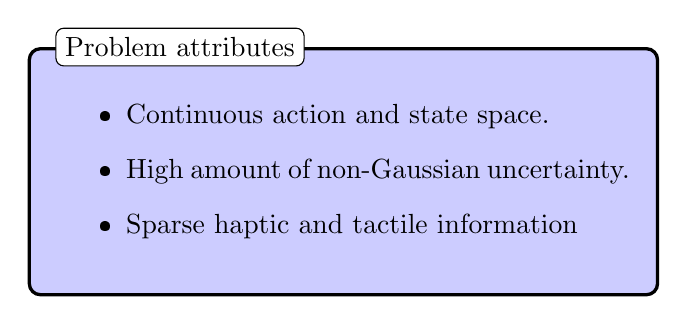
\begin{tikzpicture}
\node [fancy_box] (box){
\begin{minipage}{0.6\textwidth}
\begin{itemize}
 \item Continuous action and state space.
 \item High amount of non-Gaussian uncertainty.
 \item Sparse haptic and tactile information
\end{itemize}
\end{minipage}
};
\node[fancytitle, right=10pt] at (box.north west) {Problem attributes};
\end{tikzpicture}
\end{center}

Our approach relies on the assumption that humans are sufficiently good at handling uncertainty, that their behaviour can be learned and 
transferred to an artificial agent. A traditional PbD approach has a teacher demonstrate a task during which the state of the robot
(joint or Cartesian position) and applied actions (velocities) are recorded and stored as a dataset $D=\{(x,a)\}$. From this dataset a 
regression policy is learned $\policy(x,a)$ which encapsulates the behaviour. The policy after being learned can be refined via policy search if wanted. 
In a POMDP setting however, the state is not known and is instead represented by a belief state, $b$. In this thesis we follow the
PbD approach, gather a set of demonstrations of belief states and actions $\{(b,a)\}$ and learn a generative distribution $\policy(b,a)$
of the behaviour which can then transfer to a robot. There are a few caveats which make this task not as straight forward as it seams.

\begin{itemize}
 \item \textbf{The belief state is unknown}: When the robot apprentice is watching the human perform a search task under state uncertainty, it is 
 unable to observe the belief state of the human. All that the agent can observe directly are the actions of the teacher. We make two assumptions, the first 
 is that apprentice can infer the observations of the teacher by examining the teachers relation with the environment and secondly the initial uncertainty of the 
 teacher is assumed to be known. From these two assumptions, the sequence of belief states can be inferred via a Bayesian filter. This implies that  the mental 
 belief state of the human teacher is in fact known given the assumptions. We give more details in Chapter 3 on the validity of this assumption
 in which will discuss the relation it has with Bayesian Theory of Mind (BoTM).
 
 \item \textbf{Learning a policy as a function of non-parametric beliefs:} Given that we are considering high levels of uncertainty and type of observations are sparse
 and in the form of contacts, no parametrisation of the belief in terms of a Gaussian function would be adequate. In this thesis all the considered beliefs will be from the non-parametric 
 Bayesian filter family, such as particle filters, which allows for a lot of flexibility. Learning a policy directly as a function of a particle filter is intractable. First 
 in non-parametric filters there is typically thousands of states and in efficient particle filters the number of parameters varies over time. We take a from of \textbf{belief compression}
 in which transform the belief into the most likely state and the entropy. In this way the size of the belief state is fixed and low dimensional.
 
 \item \textbf{Reactive policy}: The control loop which computes a belief state, compresses, and computes the 
 resulting action to take should happen at around 10 to 100 Hz. This range may seem arbitrary but is in fact based on the humans control ability which at the highest
 cognitive level a delay in response is around 100ms and at the lowest reflex level at around 10-20 ms \cite{Biomechanics_2009}. This is to draw attention that the 
 full control loop, belief filtering, compression and action prediction should all happen within this range.
 
 \item \textbf{Scalable belief filter}: In scenarios in which there are multiple objects being searched for by a human teacher, the joint belief distribution 
 of a non-parametric Bayesian state space filter will become quickly computationally intractable. This motivates the development of a new type of SLAM filter methods
 which can scale in situations in which observations are very sparse.
\end{itemize}


\begin{figure}
 \centering
 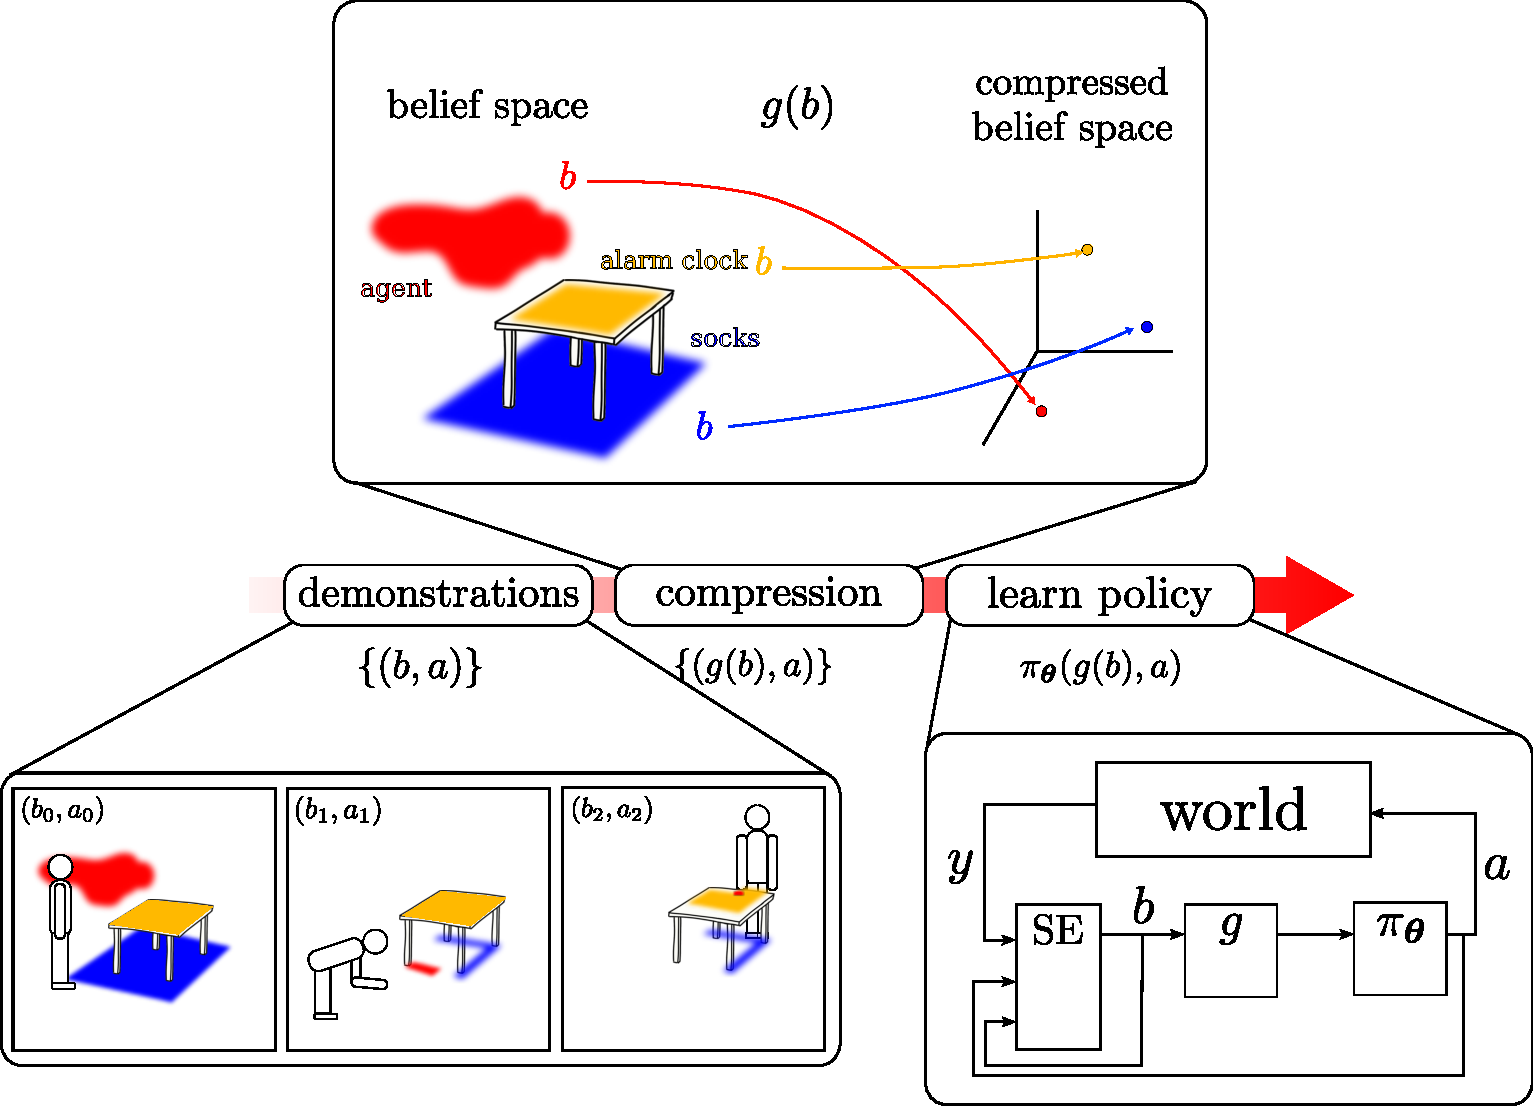
\includegraphics[width=\textwidth]{./ch2-Background/Figures/approach_concept.pdf}
 \caption{Three stages of learning a POMDP policy from human demonstrations. \textbf{Demonstrations:} An apprentice is looking at a human teacher who is searching for the
 alarm clock's button and his pair of socks. The agent assumes a priori the beliefs the human has with respect to his position and that of the alarm clock and socks, these are 
 represented by the red, yellow and blue density functions. \textbf{Compression:} Given the data set of beliefs and actions obtained from the demonstrations, the beliefs 
 is compressed to a fixed parametrisation. \textbf{Learn policy:} A generative policy, $\policy(g(b),a)$ is learned from the actions and compressed beliefs and can be executed 
 according the schematic on the right. SE represents any Bayesian state space estimator, which takes as input, the current observation, belief and action and outputs the next 
 belief state.}
\end{figure}


